\documentclass[12pt]{report}





\usepackage[margin= 1in]{geometry}
\usepackage{article_macros}


\sloppy
\allowdisplaybreaks



\newcommand{\cas}{\mathrm{cas}}
\newcommand{\cht}{\mathsf{H}}
\newcommand{\qht}{\mathsf{QHT}}
\newcommand{\cft}{\mathsf{F}}
\newcommand{\qft}{\mathsf{QFT}}
\newcommand{\comph}{\mathsf{cmpIndex}}
\newcommand{\gen}{\mathsf{Gen}}
\newcommand{\ver}{\mathsf{Ver}}




\definecolor{citecolor}{HTML}{009933}

\hypersetup{
	unicode = true,
    colorlinks = true,
    citecolor = blue,
    filecolor = blue,
    linkcolor = blue,
    urlcolor = blue,
    pdfstartview = {FitH},
}





\title{
  \textbf{Quantum Walks and Application to Quantum Money}\\[2em]
  \normalsize by\\[2em]
  \text{\large Ali Mousavi} \\[5em]
  \text{\shortstack{A Master's Thesis \\[0.5em]
   Submitted to the Department of Computing and Software\\[0.5em]
   McMaster University\\[0.5em]
   In Fulfillment of the Requirements\\[0.5em]
   For a Master's Degree}
  }

}


\date{April 2025}







\begin{document}




\maketitle
\tableofcontents


\newpage
\textbf{\large Abstract}\\


This thesis explores the foundations of quantum computation, focusing on quantum walks and their application to quantum money. Quantum walks, particularly continuous-time quantum walks based on group actions, serve as a powerful computational tool with applications in search algorithms and cryptographic protocols. We examine their mathematical structure and their advantages over classical random walks, emphasizing their efficiency in state evolution and probability distribution spreading. As a part of this work, we examine efficient implementations of transforms such as the Quantum Fourier Transform ($\qft$) and the Quantum Hartley Transform ($\qht$), analyzing their role in encoding quantum states for secure cryptographic applications. In particular, we discuss a novel instantiation of a quantum money scheme based on $\qht$, leveraging its unique properties for improved security and efficiency.
To ensure the robustness of this quantum money scheme, we develop a verification mechanism utilizing quantum walks. Unlike previous approaches, which rely on standard quantum state measurements, our method employs continuous-time quantum walks to authenticate quantum money, preventing counterfeiting while maintaining computational feasibility. Additionally, we present a detailed discussion on the efficient implementation of this scheme, including optimized circuit designs and error mitigation strategies.








\chapter{Introduction}
Quantum money, first introduced in a seminal paper by Wiesner~\cite{Wiesner1983}, is a form of currency represented by quantum states. Unlike classical money, an ideal quantum bill cannot be counterfeited due to the no-cloning theorem of quantum mechanics, which prohibits making an identical copy of an unknown quantum state. Wiesner’s original scheme (now termed a \emph{private-key quantum money} scheme) had significant practical drawbacks: it required the issuing bank’s secret key to verify each banknote, meaning the bank had to be involved in every transaction. This reliance on the bank for verification severely limits the usability of private-key quantum money schemes.

In 2009, Aaronson~\cite{Aaronson2009} proposed the first \emph{public-key quantum money} scheme, in which anyone can verify a quantum banknote while only the bank can generate new valid banknotes. Public-key quantum money removes the transactional bottleneck of involving the bank every time. Aaronson’s specific scheme was later broken by Lutomirski et al.~\cite{Lutomirski2010}. In the years since, several alternative public-key quantum money constructions have been explored. However, each of these proposals has either been broken by further cryptanalysis or relies on unconventional cryptographic assumptions, making their security or practicality questionable.

\medskip\noindent\textbf{Quantum Money from Group Actions and the Fourier Transform.} 
A promising candidate for secure public-key quantum money based on more standard assumptions was recently proposed by Zhandry~\cite{Zhandry2022}. In Zhandry’s scheme, the core idea is to use an abelian group action as the foundation for the quantum state. Each money state (quantum banknote) is prepared as a \emph{group-action Fourier state}, and the corresponding serial number is an element of the underlying group (we will elaborate on these terms in later chapters). The verification algorithm in this scheme uses a group-action phase kickback routine to extract the serial number from the quantum banknote and check its validity. Doliskani~\cite{Doliskani2023} later proved that Zhandry’s scheme is secure in the generic group action model, providing evidence for its security under well-defined assumptions.

\medskip\noindent\textbf{This Work – Motivation and Contributions.} 
In this thesis, we adapt Zhandry’s group-action quantum money scheme by replacing its use of the Quantum Fourier Transform with the \emph{Quantum Hartley Transform} ($\qht$) over finite abelian groups. The motivation behind this substitution is multifold. First, using the Hartley transform causes the banknotes to have \emph{real} amplitudes instead of complex amplitudes. We believe this shift from complex to real quantum states may offer both computational and theoretical advantages. For example, certain mathematical identities hold for any two real orthonormal bases that do not generally hold for complex bases; such differences can affect the properties of quantum states and were a barrier in prior analyses (indeed, an attempted “quantum lightning” construction in \cite{Zhandry2022} failed due to properties of complex phases that do not arise with real amplitudes). Beyond this specific context, our work is a first step toward employing real-valued quantum transforms in quantum cryptography and quantum algorithms. To the best of our knowledge, this is the first significant quantum cryptographic construction that makes essential use of the quantum Hartley transform. We hope that exploring real-amplitude quantum states will inspire further research into new quantum algorithms and optimizations for real-valued transforms.

We now summarize our main contributions:
\begin{itemize}
    \item We propose a new \textbf{public-key quantum money scheme} based on abelian group actions and the quantum Hartley transform. This scheme is an adaptation of Zhandry’s group-action money scheme, modified to output real-amplitude quantum states. 
    \item When using the Hartley transform instead of the Fourier transform, the original verification method from Zhandry’s scheme is no longer straightforward and requires the use of twists to function correctly. Instead, we offer a more direct verification approach based on quantum walks.
    \item We show that the serial number associated with a money state (which is a hidden group element) can be efficiently computed from the quantum state. In particular, we develop a \textbf{continuous-time quantum walk algorithm} to extract the serial number of a given banknote state. This algorithm leverages the structure of the group action and the spectral properties of an associated Cayley graph. Our method demonstrates that one can recover the hidden group element (serial) with high success probability, which not only underpins the new verification technique but is also of independent interest.
    \item In the course of our construction, we introduce a new algorithm for efficiently implementing the \textbf{quantum Hartley transform} and related real transforms. We present a recursive technique that exploits the structure of the Hartley transform, yielding a lower gate complexity than prior approaches in the literature.
\end{itemize}

In summary, our work combines ideas from quantum cryptography (public-key quantum money), quantum walks, and quantum signal processing (Hartley and related transforms) to create a novel and potentially practical quantum money scheme. 

\medskip\noindent\textbf{Thesis Organization.} 
The remainder of this thesis is organized as follows. In Chapter~\ref{chap:backgound}, we provide background on the basics of quantum computation and the theory of group actions, including the concept of cryptographic group actions which underlie our money scheme. Chapter~\ref{chap:quantum_walks} covers quantum walks, both continuous-time and discrete-time, outlining their differences and importance in quantum algorithms. In Chapter~\ref{chap:simulating}, we apply the quantum walk framework to group actions: we describe how a continuous-time quantum walk on a group action can be simulated efficiently, a crucial step for our serial number extraction algorithm. Chapter~\ref{chap:quantum_money} details the quantum money scheme itself and the role of the Hartley transform in its construction. We explain how the scheme is formulated and discuss the advantages and challenges introduced by using the Hartley transform. Finally, Chapter~\ref{chap:verification} presents the verification algorithm for the Hartley-based quantum money. This chapter shows how we use quantum walks (as developed in Chapter 4) to reliably verify banknotes and compute their serial numbers, thereby addressing the verification issues that arose from the use of real amplitudes.
\vspace{1em}



\chapter{Background of Quantum Computation and Group Actions}\label{chap:backgound}



\section{Quantum Computation Basics}


Quantum computation is a model of information processing rooted in the principles of quantum mechanics. Unlike classical systems, which encode and manipulate information using deterministic bits, quantum systems store information in quantum states—vectors in complex Hilbert spaces—that can exhibit phenomena with no classical analogue. The most notable of these are \emph{superposition}, which allows quantum systems to be in multiple configurations simultaneously, and \emph{entanglement}, which enables correlations between parts of a system that cannot be explained classically. These characteristics endow quantum computers with computational abilities that can outperform classical counterparts in certain tasks. For a comprehensive introduction to quantum computation and quantum information we refer the reader to ~\cite{NielsenChuang2010, watrous2018theory, kaye2006introduction}.

To rigorously define the framework of quantum computation, we begin with some basic notation. Let $\mathcal{H}$ be a finite-dimensional Hilbert space over the complex numbers. This space is equipped with an inner product and an orthonormal basis $\{\ket{s} : s \in S\}$, where $S$ is a finite index set that corresponds to the classical configurations of the system. Each element $\ket{s} \in \mathcal{H}$ represents a quantum basis state, analogous to a classical state. A general quantum state $\ket{\alpha} \in \mathcal{H}$ is a unit vector, and can be expressed as a linear combination of the basis vectors:
\[
\ket{\alpha} = \sum_{s \in S} a_s \ket{s}, \qquad \text{where } a_s \in \mathbb{C}, \quad \sum_{s \in S} |a_s|^2 = 1.
\]
Here, the complex numbers $a_s$ are called \emph{amplitudes}, and the squared magnitudes $|a_s|^2$ correspond to the probabilities of observing the state $\ket{s}$ upon measurement. The inner product between two states $\ket{\alpha}$ and $\ket{\beta}$ is denoted by $\bra{\beta}\alpha\rangle$, where $\bra{\alpha}$ is the conjugate transpose (or Hermitian adjoint) of the $\ket{\alpha}$.

The most elementary quantum system is the \emph{qubit}, or quantum bit, which corresponds to a unit vector in the two-dimensional Hilbert space $\mathbb{C}^2$. In the computational basis $\{\ket{0}, \ket{1}\}$, any pure state of a qubit can be written as
\[
\ket{\psi} = \alpha \ket{0} + \beta \ket{1}, \qquad \text{where } \alpha, \beta \in \mathbb{C}, \quad |\alpha|^2 + |\beta|^2 = 1.
\]
Unlike a classical bit, which must be either 0 or 1, a qubit can exist in a superposition of both states simultaneously. The ability to process such coherent superpositions is one of the key features that distinguishes quantum computation from classical models.

When considering multiple qubits, the joint state of the system resides in the \emph{tensor product} of the individual Hilbert spaces. For example, a system of $n$ qubits is described by the space
\[
\mathcal{H} = \left( \mathbb{C}^2 \right)^{\otimes n} \cong \mathbb{C}^{2^n}.
\]
The standard basis for this space consists of all computational basis states $\ket{x}$ where $x \in \{0,1\}^n$ is a bit string of length $n$. A general pure state of $n$ qubits is then written as
\[
\ket{\Psi} = \sum_{x \in \{0,1\}^n} \alpha_x \ket{x}, \qquad \sum_{x} |\alpha_x|^2 = 1.
\]
Because of the exponential growth in the dimension of the Hilbert space with the number of qubits, quantum systems can store and process information in ways that are exponentially more efficient (in terms of representation) than classical systems. Additionally, this tensor product structure enables the existence of \emph{entangled states}—those which cannot be factored into product states of individual qubits. Entanglement plays a crucial role in quantum algorithms, communication, and cryptography.

The formal behavior of quantum systems is governed by a small set of postulates that form the mathematical foundation of quantum mechanics. These postulates determine how quantum systems are represented, how they evolve, and how observations are made.

\begin{enumerate}
  \item \textbf{State Space.} Every isolated physical system is associated with a Hilbert space $\mathcal{H}$, and its state is described by a unit vector $\ket{\psi} \in \mathcal{H}$. For composite systems composed of subsystems $A$ and $B$, the state space is the tensor product $\mathcal{H}_A \otimes \mathcal{H}_B$. If $\{\ket{a_i}\}$ and $\{\ket{b_j}\}$ are orthonormal bases for $\mathcal{H}_A$ and $\mathcal{H}_B$, then $\{\ket{a_i} \otimes \ket{b_j}\}$ forms an orthonormal basis for the joint system.

  \item \textbf{Unitary Evolution.} The evolution of a closed quantum system is described by a unitary transformation. If the system is in state $\ket{\psi}$ at some initial time, then at a later time it evolves to $\ket{\psi'} = U \ket{\psi}$, where $U$ is a unitary operator satisfying $U^\dagger U = U U^\dagger = I$. This ensures that the norm of the state vector—and hence the total probability—is preserved under evolution.

  \item \textbf{Measurement.} Measurement is a probabilistic process governed by an orthonormal basis $\{\ket{s}\}_{s \in S}$ of $\mathcal{H}$. When a measurement is performed on a state $\ket{\alpha} = \sum_{s \in S} a_s \ket{s}$, the outcome is some $s \in S$ with probability $|a_s|^2$, and the system collapses to the corresponding basis state $\ket{s}$. This probabilistic rule is known as the Born rule. Measurement is not reversible: it fundamentally alters the state and discards phase and superposition information not aligned with the measured basis.

  \item \textbf{Composition of Systems.} If two quantum systems \( A \) and \( B \) are described by Hilbert spaces \( \mathcal{H}_A \) and \( \mathcal{H}_B \), respectively, then the combined system is described by the tensor product \( \mathcal{H}_A \otimes \mathcal{H}_B \). A product state of the form \( \ket{\psi_A} \otimes \ket{\psi_B} \) represents a system where \( A \) and \( B \) are uncorrelated. In general, however, the state may be entangled, and cannot be written as a product of subsystems.

  If unitary operators \( U_A \) and \( U_B \) act on \( \mathcal{H}_A \) and \( \mathcal{H}_B \), respectively, then the combined unitary \( U_A \otimes U_B \) acts on the joint system by applying \( U_A \) to subsystem \( A \) and \( U_B \) to subsystem \( B \), independently. That is,
  \[
  (U_A \otimes U_B)(\ket{\psi_A} \otimes \ket{\psi_B}) = (U_A \ket{\psi_A}) \otimes (U_B \ket{\psi_B}).
  \]
  This operation preserves the separability of product states, and more generally, acts linearly on the full Hilbert space \( \mathcal{H}_A \otimes \mathcal{H}_B \).



\end{enumerate}

Together, these postulates define the operational behavior of quantum systems and underpin the structure of quantum computation. The state space formalism allows for the representation of complex probabilistic and entangled phenomena, while unitary evolution enables coherent manipulation of information. Measurement introduces irreversibility and classical output, allowing for the extraction of computational results from quantum processes. Finally, the tensor product composition rule enables scalable modeling of multipartite systems and is the mathematical basis for the power of quantum algorithms.


\section{Classical vs Quantum Computation}


In classical computation, circuits are composed of wires and logic gates, such as AND, OR, and NOT, that act on bits—elements of $\{0,1\}$. These logic gates are inherently irreversible: for example, given the output of an OR gate, one cannot deduce the exact inputs. In contrast, quantum computation operates under the strict constraint that all operations must be unitary, and therefore \emph{reversible}.

Quantum computers are built from quantum circuits, which consist of wires (representing qubits) and quantum gates (unitary operations). Qubits may exist in superpositions of basis states and, when acted upon by quantum gates, evolve linearly in accordance with the postulates of quantum mechanics.

Unlike classical gates that map fixed bitstrings to other bitstrings, quantum gates are linear operators acting on vectors in complex Hilbert space. For a single qubit, this means that gates must preserve the inner product and norm of quantum states. Hence, quantum gates must be represented by unitary matrices $U$ such that $U^\dagger U = I$.

\subsection{Elementary Quantum Gates}

Many single-qubit quantum gates have no classical counterparts. A few key examples include:

\begin{itemize}
  \item \textbf{Pauli-X (NOT) Gate:} Acts as the quantum analog of the classical NOT gate.
  \[
  X = \begin{bmatrix} 0 & 1 \\ 1 & 0 \end{bmatrix}, \quad X \ket{0} = \ket{1}, \quad X \ket{1} = \ket{0}
  \]
  
  \item \textbf{Pauli-Y Gate:} Introduces a $\pi$-rotation around the $y$-axis of the Bloch sphere.
  \[
  Y = \begin{bmatrix} 0 & -i \\ i & 0 \end{bmatrix}
  \]

  \item \textbf{Pauli-Z Gate:} Flips the sign of the $\ket{1}$ component.
  \[
  Z = \begin{bmatrix} 1 & 0 \\ 0 & -1 \end{bmatrix}
  \]

  \item \textbf{Hadamard Gate (H):} Places a qubit into an equal superposition of $\ket{0}$ and $\ket{1}$.
  \[
  H = \frac{1}{\sqrt{2}} \begin{bmatrix} 1 & 1 \\ 1 & -1 \end{bmatrix}
  \]
  This gate transforms:
  \[
  \ket{0} \mapsto \frac{\ket{0} + \ket{1}}{\sqrt{2}}, \quad \ket{1} \mapsto \frac{\ket{0} - \ket{1}}{\sqrt{2}}
  \]

  \item \textbf{Phase Gate (S):} Applies a $\frac{\pi}{2}$ phase to $\ket{1}$:
  \[
  S = \begin{bmatrix} 1 & 0 \\ 0 & i \end{bmatrix}
  \]

  \item \textbf{$\pi/8$ Gate (T):} Applies a phase of $\pi/4$:
  \[
  T = \begin{bmatrix} 1 & 0 \\ 0 & e^{i\pi/4} \end{bmatrix}
  \]
  It is the square root of the Phase gate and thus the fourth root of $Z$.
\end{itemize}

These gates are all unitary and form the building blocks of single-qubit quantum circuits.

\subsection{Controlled Gates and Universality}

Quantum computation requires not only single-qubit gates, but also multi-qubit gates that enable interactions between qubits. The most fundamental among these is the \emph{Controlled-NOT (CNOT)} gate. This two-qubit gate flips the target qubit if and only if the control qubit is in the state $\ket{1}$. In matrix form, and with respect to the computational basis $\{\ket{00}, \ket{01}, \ket{10}, \ket{11}\}$, it is given by
\[
\text{CNOT} = 
\begin{bmatrix}
1 & 0 & 0 & 0 \\
0 & 1 & 0 & 0 \\
0 & 0 & 0 & 1 \\
0 & 0 & 1 & 0 \\
\end{bmatrix}.
\]
The CNOT gate plays a central role in quantum algorithms and is essential for generating entangled states. It serves as the quantum analogue of the classical XOR gate. A natural generalization of the CNOT is the family of controlled-$U$ gates, where $U$ is any single-qubit unitary. A controlled-$U$ gate applies $U$ to the target qubit only when the control qubit is $\ket{1}$; otherwise, it acts as the identity. This construction is a key component in many quantum algorithms, including quantum phase estimation and Shor’s algorithm.

In classical computation, the set of gates $\{\text{AND}, \text{NOT}\}$ is universal, meaning any Boolean function can be computed using only these gates. Analogously, in the quantum setting, certain sets of gates are \emph{universal for quantum computation}. That is, they can approximate any unitary transformation on any number of qubits to arbitrary precision. A particularly important universal gate set is $\{H, T, \text{CNOT}\}$, consisting of the Hadamard gate, the $\pi/8$ gate (also called the $T$ gate), and the CNOT gate. This set forms the basis for fault-tolerant quantum computing and is sufficient to construct any quantum algorithm.

Unlike classical circuits, quantum circuits must obey the constraints of reversibility and linearity. They are acyclic and do not allow for operations like signal fanout or feedback loops. One key difference from classical logic is the restriction imposed by the \emph{no-cloning theorem}, which states that it is impossible to create a perfect copy of an arbitrary unknown quantum state. This makes operations like classical bit copying or broadcasting fundamentally incompatible with quantum mechanics. Moreover, measurement in quantum mechanics is inherently irreversible. When a qubit is measured in the computational basis, its state collapses probabilistically to either $\ket{0}$ or $\ket{1}$, with probabilities determined by the squared magnitudes of its amplitudes. The outcome is a classical bit, and the original quantum superposition is lost in the process.

To illustrate these concepts, consider the task of swapping the quantum states of two qubits. This seemingly simple operation cannot be accomplished directly but can be implemented by a specific sequence of three CNOT gates. Given two qubits in states $\ket{a}$ and $\ket{b}$, the SWAP operation is performed via the sequence
\[
\text{CNOT}_{1,2} \rightarrow \text{CNOT}_{2,1} \rightarrow \text{CNOT}_{1,2},
\]
which effectively interchanges the states, resulting in $\ket{b} \ket{a}$. This example highlights how even basic classical-like operations must be constructed carefully using reversible building blocks in the quantum circuit model.




\section{Group Actions in Cryptography}
At the heart of our quantum money scheme is the notion of a group action. A \textbf{group action} of a group $G$ on a set $X$ is a function $*\colon G \times X \to X$ that satisfies two properties: (1) the identity element $e \in G$ acts trivially on every $x \in X$ ($e * x = x$), and (2) the action is compatible with the group operation, meaning $g*(h* x) = (gh)*x$ for all $g,h \in G$ and $x \in X$. We will denote the result of $g$ acting on $x$ by $g*x$.

The orbit of an element $x \in X$ under the action is the set $G * x = \{g*x : g \in G\} \subseteq X$. If there is exactly one orbit (i.e., $G * x = X$ for some $x$), the action is called \emph{transitive}. If, in addition, no non-identity group element fixes any $x$ (i.e., $g * x = x$ implies $g = e$), then the action is \emph{free}. A group action that is both transitive and free is sometimes called a \textbf{regular action}. In a regular action, for any two elements $y, z \in X$, there is a unique group element $g$ such that $g * y = z$. In other words, $G$ acts like a permutation group that moves elements of $X$ around, and knowing the starting and ending point uniquely determines the “move” $g$. In this case $|X| = |G|$, and we can think of $X$ as essentially a copy of $G$ with the group structure “hidden” by the action.

Group actions are ubiquitous in modern cryptography. A \textbf{cryptographic group action} ~\cite{Castryck2020} is one where the action is easy to compute in the forward direction, but inverting the action (recovering $g$ from $x$ and $g*x$) is computationally hard. This essentially functions as a one-way function: given $x$ and $g$, it is easy to compute $y = g*x$, but given $x$ and $y$ it is infeasible to find $g$ (except with negligible probability). One classical example is the discrete logarithm problem: consider the cyclic group $G = \mathbb{Z}_p^*$ (the multiplicative group of a prime field) acting on itself by exponentiation. Let $X = G$ and define $g * x = x^g \pmod p$ (treating group elements as integers). Here $g$ is an exponent. This is a group action (in fact, just the group’s own operation written differently), and computing $x^g \bmod p$ is efficient. However, given $x$ and $y = x^g$, finding $g$ requires solving a discrete log problem, which is believed to be hard for suitable choices of $p$. Thus, exponentiation can be viewed as a one-way group action.

Another prominent example comes from elliptic-curve cryptography: the action of an ideal class group on a set of elliptic curves. In schemes like CSIDH (Commutative Supersingular Isogeny Diffie–Hellman), an abelian group of ideal classes $G$ acts on the set $X$ of supersingular elliptic curves by isogeny (an isogeny is a structure-preserving map between curves). Starting from a curve $x_0$, one can efficiently compute $g * x_0$ (which is another elliptic curve) for any group element $g$, but given two curves $x_0$ and $x = g * x_0$, it is believed to be computationally hard to recover $g$. This hard problem is the foundation of isogeny-based cryptography. We refer to such $G$ and $X$ as a \emph{cryptographic group action} pair.

Cryptographic group actions provide a natural platform for public-key quantum money schemes. In such schemes, the secret “serial number” of a quantum banknote can be an element $h \in G$, and the quantum state of the banknote can be some function of $h*x_0$ for a public base point $x_0 \in X$. The hardness of inverting the action ($x_0$ and $x = h*x_0$ do not easily reveal $h$) contributes to the security against counterfeiting, while the structure of the group action can be used to efficiently verify authenticity (as we will see with the Fourier or Hartley transform techniques).

We will assume throughout that we have a family of abelian group actions $(G,X)$ that are cryptographically suitable: $|G|$ is large (growing with the security parameter), the action is efficiently computable, transitive and free (so $|X|=|G|$), and inverting the action is infeasible without the secret key. Such families are conjectured to exist (for example, the isogeny-based actions, and others discussed in cryptographic literature). 

Finally, we note that working in the \textbf{generic group model} (or generic group \emph{action} model) is a common theoretical approach to analyze security. In a generic model, the group elements are treated as black-box labels without exploiting any special algebraic structure beyond group axioms. Doliskani’s proof of security for Zhandry’s scheme [15] was in such a generic model for group actions, lending confidence that no “generic” attack can break the scheme. In this thesis, we focus on designing the scheme and algorithms at a high level and assume the underlying group action is secure; a detailed security proof is beyond our scope, though we rely on prior results for reassurance.








\section{The Quantum Fourier Transform}
The \textit{Quantum Fourier Transform $\qft$} is a quantum analogue of the classical discrete Fourier transform and plays a fundamental role in many quantum algorithms, including Shor’s factoring algorithm and quantum phase estimation. It enables the transformation of quantum states into the frequency domain, revealing periodicities and structure that may be hidden in the computational basis.

A common instance of the $\qft$ is over the cyclic group \( \mathbb{Z}_N  = \{0,1,...,N-1\}\). Given a state \( \ket{x} \in \mathbb{C}^N \), the $\qft$ over \( \mathbb{Z}_N \) maps it to
\[
\ket{x} \mapsto \frac{1}{\sqrt{N}} \sum_{k=0}^{N-1} e^{2\pi i xk / N} \ket{k}.
\]
When \( N = 2^n \), we can express the index \( x \) in binary as \( x = j_1 j_2 \ldots j_n \), where \( x = j_1 2^{n-1} + j_2 2^{n-2} + \cdots + j_n \). In this case, the $\qft$ has a beautiful product representation:
\[
\ket{j_1 \cdots j_n} \mapsto \frac{1}{2^{n/2}} \bigotimes_{k=1}^n \left( \ket{0} + e^{2\pi i 0.j_k j_{k+1} \cdots j_n} \ket{1} \right),
\]
where \( 0.j_k j_{k+1} \cdots j_n \) denotes the binary fraction \( \frac{j_k}{2} + \frac{j_{k+1}}{4} + \cdots + \frac{j_n}{2^{n-k+1}} \). This form reveals the tensor product structure of the $\qft$: the transformed state decomposes as a product of single-qubit superpositions, each involving successively finer phase rotations.

This structure allows for an efficient quantum circuit implementation. The circuit consists of a sequence of Hadamard gates and controlled phase gates \( R_k = \begin{bmatrix} 1 & 0 \\ 0 & e^{2\pi i / 2^k} \end{bmatrix} \), followed by a series of swap gates to reverse the order of qubits. For each qubit \( j_k \), a Hadamard gate is applied first, followed by controlled-\( R_2, R_3, \ldots \) gates from subsequent qubits. The number of gates required is \( \Theta(n^2) \), making the $\qft$ over \( 2^n \) dimensions efficiently implementable on a quantum computer \cite[Section 5.1]{NielsenChuang2010}.

In this work, we extend the notion of the $\qft$ to more general finite groups beyond \( \mathbb{Z}_N \). This generalization is essential for studying quantum walks on group-based graphs and analyzing quantum algorithms defined over non-abelian structures.


Let $G$ be an abelian group. The group of characters of $G$, denoted $\hat{G}$, consists of homomorphisms of the form $\chi(a, \cdot): G \to \mathbb{C}$ for each $a \in G$. If the group has the structure $G \cong \mathbb{Z}_{N_1} \oplus \cdots \oplus \mathbb{Z}_{N_k}$, then the character function $\chi(a, \cdot)$ can be expressed explicitly as
\[
\chi(a, x) = \omega_{N_1}^{a_1x_1} \cdots \omega_{N_k}^{a_kx_k}
\]
where $\omega_M = \exp(2\pi i / M)$ is a primitive $M$-th root of unity. Given a function $f: G \to \mathbb{C}$, its Fourier transform is defined as
\[
\hat{f}(a) = \frac{1}{\sqrt{\abs{G}}} \sum_{x \in G} \chi(a, x) f(x).
\]
Correspondingly, the quantum Fourier transform of a normalized state $\sum_{g \in G} f(g) \ket{g}$ is given by $\sum_{x \in G} \hat{f}(x) \ket{x}$. The $\qft$ over \( G \) is simply a tensor product of $\qft$s over each \( \mathbb{Z}_{N_i} \), and can therefore be implemented efficiently.


Now consider a regular group action $(G, X, *)$. For any subset $S \subseteq G$, element $y \in X$, and $h \in G$, we define the following state:
\begin{equation}
    \label{eq:x-fourier-basis}
    \ket{S^{(h)} * y} = \frac{1}{\sqrt{\abs{S}}} \sum_{g \in S} \chi(g, h) \ket{g * y}.
\end{equation}
The vector space $\mathbb{C}^X$ has two natural orthonormal bases. The first is the standard basis $\{\ket{x} : x \in X\}$, which, for any fixed $x \in X$, can be written as $\{\ket{g * x} : g \in G\}$ because the regularity of the action implies a bijection between $G$ and $X$ (i.e., $|G| = |X|$). The second basis consists of the following quantum states:
\[
\ket{G^{(h)} * x} = \frac{1}{\sqrt{\abs{G}}} \sum_{g \in G} \chi(g, h) \ket{g * x}, \quad h \in G.
\]
These states are simultaneous eigenvectors of the group action unitaries. Specifically, for each $k \in G$, let $U_k$ denote the unitary operator defined by $U_k \ket{y} = \ket{k * y}$. Then we have:
\[
U_k \ket{G^{(h)} * x} = \chi(-k, h) \ket{G^{(h)} * x}.
\]
This property makes the states $\ket{G^{(h)} * x}$ analogous to Fourier states over the abelian group $G$, and we will often refer to them as such.


\section{The Quantum Hartley Transform}

Another concept we use is the \textbf{quantum Hartley transform} ($\qht$), which replaces complex exponentials with real sinusoidal kernels.
Let $N$ be a positive integer, and let $\Z_N$ denote the additive cyclic group of integers modulo $N$. The Hartley transform of a function $f: \Z_N \to \R$ is defined as the function $\cht_N(f): \Z_N \to \R$ given by
\[
\cht_N(f)(a) = \frac{1}{\sqrt{N}} \sum_{y = 0}^{N - 1} \cas\Big(\frac{2 \pi ay}{N}\Big) f(y),
\]
where $\cas(x) = \cos(x) + \sin(x)$. Similar to the Fourier transform, $\cht_N$ is a linear operation, and one can verify that it is unitary. This definition extends naturally to general abelian groups. Suppose $G = \Z_{N_1} \oplus \Z_{N_2} \oplus \cdots \oplus \Z_{N_k}$ is a decomposition of an abelian group into cyclic components. For a function $f: G \to \R$, the Hartley transform $\cht_G(f): G \to \R$ is defined by
\begin{equation}
    \label{eq:cht-add}
    \cht_G(f)(a_1, \dots, a_k) = \frac{1}{\sqrt{\abs{G}}} \sum_{y_1 = 0}^{N_1 - 1} \cdots \sum_{y_k = 0}^{N_k - 1} \cas\Big(\frac{2 \pi a_1y_1}{N_1} + \cdots + \frac{2 \pi a_ky_k}{N_k}\Big) f(y_1, \dots, y_k),
\end{equation}
with $(a_1, \dots, a_k) \in G$. Introducing the notation $\alpha(\bm{y}) = y_1 / N_1 + \cdots + y_k / N_k$, a more concise form for $\cht_G$ is
\[
\cht_G(f)(\bm{a}) = \frac{1}{\sqrt{\abs{G}}} \sum_{\bm{y} \in G} \cas(2\pi \lrang{\bm{a}, \alpha(\bm{y})}) f(\bm{y}).
\]

Using the identity
\[
\cas(2\pi \lrang{\bm{a}, \alpha(\bm{y})}) = \frac{1 - i}{2}\chi(\bm{a}, \bm{y}) + \frac{1 + i}{2}\chi(-\bm{a}, \bm{y}),
\]
it follows that
\begin{equation}
    \label{eq:ht-ft}
    \cht_G = \frac{1 - i}{2}\cft_G + \frac{1 + i}{2}\cft_G^*,
\end{equation}
where $\cft_G$ denotes the Fourier transform over $G$. From this, it can be deduced that $\cht_G^2 = \mathds{1}$, confirming that $\cht_G$ is also unitary. An alternative version of the Hartley transform, often appearing in literature, is the multiplicative variant defined by
\begin{equation}
    \label{eq:cht-mult}
    \cht_G(f)(a_1, \dots, a_k) = \frac{1}{\sqrt{\abs{G}}} \sum_{y_1 = 0}^{N_1 - 1} \cdots \sum_{y_k = 0}^{N_k - 1} \mathrm{cas}\Big(\frac{2 \pi a_1y_1}{N_1}\Big) \cdots \cas\Big(\frac{2 \pi a_ky_k}{N_k}\Big) f(y_1, \dots, y_k).
\end{equation}
This transform is also unitary, as demonstrated in the following lemma.

\begin{lemma}
    The Hartley transform \eqref{eq:cht-mult} is unitary.
\end{lemma}

\begin{proof}
    Consider the function $f$ as a vector indexed by the elements of $G$. The matrix associated with $\cht_G$ is the tensor product of the matrices corresponding to the Hartley transforms over the cyclic components $\Z_{N_i}$ of $G$. Specifically, $\cht_G = \cht_{N_1} \otimes \cht_{N_2} \otimes \cdots \otimes \cht_{N_k}$. Since each $\cht_{N_i}$ is unitary, the tensor product is also unitary, proving the claim.
\end{proof}

The quantum Hartley transform over an abelian group $G$ is given by
\begin{equation}
    \label{eq:qht}
    \qht_G: \sum_{\bm{x} \in G} f(\bm{x}) \ket{\bm{x}} \mapsto \sum_{\bm{a} \in G} \cht_G(f)(\bm{a}) \ket{\bm{a}},
\end{equation}
where normalization of the input state is omitted for brevity. The function $\cht_G(f)$ may refer to either the additive form \eqref{eq:cht-add} or the multiplicative form \eqref{eq:cht-mult}. In the special case of a single basis state $\ket{a}$ in the group $\Z_N$, the quantum Hartley transform takes the form
\begin{equation}
	\label{eq:qht-N}
	\qht_N: \ket{a} \mapsto \frac{1}{\sqrt{N}} \sum_{y = 0}^{N - 1} \cas\Big(\frac{2\pi a y}{N}\Big) \ket{y}.
\end{equation}
The unitary operator $\qht_N$ can be implemented efficiently, as will be shown in Section~\ref{sec:efficient_qht}. When using the multiplicative form~\eqref{eq:cht-mult}, the unitary $\qht_G$ decomposes as a tensor product of unitaries of the form $\qht_N$.
  

\section{Quantum Algorithms}


Quantum algorithms harness the principles of quantum mechanics to solve certain computational problems more efficiently than classical algorithms. Their power often stems from features like superposition, entanglement, and interference, which enable novel approaches to problems in search, algebra, and cryptography.

In this section, we review two fundamental quantum algorithms—the \textsf{cmpIndex} algorithm and the \textit{quantum phase estimation} algorithm—both of which will play a key role in the constructions and analyses presented in the subsequent chapters.

\paragraph{The $\comph$ algorithm.}
Suppose we are given a quantum state of the form $\ket{G^{(h)} * x}$. There exists an efficient procedure to recover the index $h$. This procedure is implemented via a unitary transformation that maps the state $\ket{G^{(h)} * x} \ket{0}$ to $\ket{G^{(h)} * x} \ket{h}$ using the technique of \emph{phase kickback}. The algorithm proceeds as follows: begin with the state $\ket{G^{(h)} * x} \ket{0}$, apply the quantum Fourier transform to the second register, and then apply the unitary operator $\sum_{k \in G} U_k \otimes \ket{k} \bra{k}$, which acts jointly on both registers. This produces the state
\[
\frac{1}{\sqrt{\abs{G}}} \sum_{k \in G} \ket{G^{(h)} * x} \chi(-k, h) \ket{k}.
\]
Finally, applying the inverse quantum Fourier transform to the second register yields the desired state $\ket{G^{(h)} * x} \ket{h}$, successfully extracting the label $h$.

\paragraph{The Phase Estimation Algorithm.}

The quantum Fourier transform lies at the heart of a powerful primitive known as \emph{quantum phase estimation}. This algorithm is fundamental to many quantum algorithms and plays a central role in problems involving eigenvalue estimation. Suppose we are given a unitary operator $U$ with an eigenvector $\ket{u}$ such that
\[
U \ket{u} = e^{2\pi i \phi} \ket{u}
\]
for some unknown phase $\phi \in [0, 1)$. The goal of the phase estimation algorithm is to estimate the value of $\phi$ to $n$ bits of precision.

Phase estimation is not only interesting as a stand-alone quantum task—estimating eigenphases of unitaries—but also serves as a key subroutine in many important quantum algorithms, such as Shor’s factoring algorithm, quantum order finding, and quantum simulations of physical systems.

The algorithm requires two quantum registers: the first (of $t$ qubits) will store the estimated phase, and the second holds the eigenvector $\ket{u}$. We assume access to a black-box unitary that performs the controlled-$U^j$ operation for any integer $j$.

\vspace{1em}
\noindent\textbf{Algorithm: Quantum Phase Estimation}
\begin{itemize}
  \item \textbf{Inputs:}
    \begin{itemize}
        \item A black box that implements controlled-$U^j$ for integer $j$.
        \item An eigenstate $\ket{u}$ of $U$, such that $U \ket{u} = e^{2\pi i \phi} \ket{u}$.
        \item $t = n + \log(2 + \frac{1}{2\epsilon})$ qubits in the first register initialized to $\ket{0}^{\otimes t}$, where $\epsilon$ is the allowed error.
    \end{itemize}
  \item \textbf{Output:} An $n$-bit approximation $\tilde{\phi}$ of $\phi$.
  \item \textbf{Procedure:}
    \begin{enumerate}
      \item Initialize the first register to $\ket{0}^{\otimes t}$ and the second register to $\ket{u}$.
      \item Apply Hadamard gates to each of the $t$ qubits in the first register to create a uniform superposition:
      \[
      \frac{1}{\sqrt{2^t}} \sum_{j=0}^{2^t - 1} \ket{j} \ket{u}.
      \]
      \item Apply the controlled-$U^j$ operation to the second register, controlled on the $j$-th basis state of the first register. This yields:
      \[
      \frac{1}{\sqrt{2^t}} \sum_{j=0}^{2^t - 1} e^{2\pi i j \phi} \ket{j} \ket{u}.
      \]
      \item Discard the second register (since it remains unchanged as $\ket{u}$) and apply the inverse quantum Fourier transform to the first register.
      \item Measure the first register. With high probability, the outcome is a $t$-bit string that approximates $\phi$ to $n$ bits of accuracy.
    \end{enumerate}
\end{itemize}

% \noindent\textbf{Runtime:} $\mathcal{O}(t^2)$ operations and a single invocation of the controlled-$U^j$ oracle for each $j$.

% \noindent\textbf{Success Probability:} At least $1 - \epsilon$.

\vspace{1em}
This procedure efficiently extracts the phase $\phi$ associated with a known eigenvector of a unitary operator and provides a foundational tool for quantum algorithms that exploit spectral properties of quantum operators. For a complete description and analysis of this algorithm, we refer the reader to \cite{NielsenChuang2010}.



\chapter{Quantum Walks -- Continuous and Discrete}\label{chap:quantum_walks}

Quantum walks are the quantum-mechanical counterparts of classical random walks on graphs. Instead of a probability distribution over vertices, a quantum walk evolves a superposition of vertex states. Interference between multiple paths leads to markedly different behavior from classical walks, often yielding faster spreading and algorithmic speedups~\cite{Aharonov2001}.

In particular, both major models of quantum walks --- continuous-time and discrete-time --- achieve \emph{ballistic spreading} (standard deviation growing linearly in time) in contrast to the diffusive $O(\sqrt{t})$ spread of classical random walks~\cite{Kempe2003}. Quantum walks have become a central framework in quantum computing, underpinning various algorithms and even universal quantum computation~\cite{Childs2009,Ambainis2003}.

In this chapter, we introduce continuous- and discrete-time quantum walks, compare their properties, and discuss their implementation on highly symmetric graphs known as Cayley graphs. We then explore how group actions and symmetry can be leveraged to analyze and construct quantum walks on these graphs.



\section{Continuous-Time Quantum Walk}


A \textbf{continuous-time quantum walk (CTQW)} is defined by a time-dependent Schrödinger equation on the vertices of a graph. Given a graph $G=(V,E)$ with $\abs{V}=N$ vertices, one assigns a basis state $\ket{j}$ to each vertex $j \in V$. The walk is governed by a Hermitian Hamiltonian $H$ that respects the graph's structure. A common choice is to take $H$ proportional to either the adjacency matrix $A$ of $G$ or the graph Laplacian $L$. For example, one may set
\[
H = \gamma A \quad \text{or} \quad H = \gamma L,
\]
where $\gamma$ is a constant coupling rate with dimensions of (time)$^{-1}$.

The Hamiltonian connects adjacent vertices: $\bra{j}H\ket{k} \neq 0$ if and only if $(j,k) \in E$. The state of the walk $\ket{\psi(t)} = \sum_{j \in V} \psi_j(t) \ket{j}$ evolves according to the Schrödinger equation:
\[
i \frac{d}{dt} \ket{\psi(t)} = H \ket{\psi(t)},
\]
with formal solution
\[
\ket{\psi(t)} = e^{-iHt} \ket{\psi(0)}.
\]

In coordinates, if we use the Laplacian $L$ defined by $L_{jk} = -\deg(j)\delta_{jk} + A_{jk}$, the equation becomes
\[
i \frac{d}{dt} \psi_j(t) = \sum_{k \in V} L_{jk} \psi_k(t),
\]
which mirrors the equation of a classical continuous-time random walk except for the factor $i$. Since $L$ (and $A$) are Hermitian, the quantum dynamics are unitary and conserve total probability (i.e., the norm of the state vector), in contrast to the irreversible nature of classical diffusion.

The continuous-time quantum walk model was first formalized by Farhi and Gutmann in 1998 as a quantum analogue of continuous Markov processes.

\subsection{Hamiltonian Choices}

One can equivalently define a CTQW using $H = A$ (the adjacency matrix) instead of the Laplacian. For an undirected $d$-regular graph, $L = dI - A$, and using $H=A$ introduces only an overall phase factor $e^{-i d t}$ in the evolution, since $dI$ contributes a global phase. Thus, on regular graphs, the choice of Laplacian versus adjacency matrix is unimportant up to a global phase. In general, the adjacency matrix is often used because it directly encodes graph connectivity. Farhi and Gutmann’s original construction corresponds to $H=A$.

Throughout this thesis, we primarily consider $H = A$ for continuous-time walks on unweighted graphs.

\subsection{Example – CTQW on a Hypercube}

The $n$-dimensional Boolean hypercube $Q_n$ is the graph on $2^n$ vertices $\{0,1\}^n$, where edges connect vertices differing in one bit. This is a $d = n$ regular graph, and can be viewed as the Cayley graph of $(\mathbb{Z}_2)^n$ with the generating set consisting of flipping each bit.

The adjacency matrix of $Q_n$ can be written as a sum of $n$ commuting terms, each acting on one bit:
\[
A_{Q_n} = \sum_{j=1}^{n} \sigma_x^{(j)},
\]
where $\sigma_x^{(j)}$ is the Pauli $X$ operator acting on the $j$-th bit (and identity on the others). Because all $\sigma_x^{(j)}$ commute, the time-evolution operator factorizes:
\[
e^{-i A_{Q_n} t} = \prod_{j=1}^{n} e^{-i \sigma_x^{(j)} t} = \bigotimes_{j=1}^{n} \left( \cos t \, I - i \sin t \, \sigma_x^{(j)} \right),
\]
yielding an analytical solution for the walk. In particular, starting from the state $\ket{0^n}$, the walker's state remains an even superposition over all vertices at Hamming distance $k$ at time $t$, with amplitudes given by the $k$-th term in the expansion of $(\cos t - i \sin t)^n$.

This shows that the quantum walk spreads across the hypercube exponentially faster than a classical random walk, which requires $O(n \log n)$ steps to approach a uniform distribution. The hypercube example illustrates how symmetry (in this case, the direct product structure) enables explicit solutions.

\subsection{Algorithmic Applications}

Continuous-time quantum walks have been employed to achieve algorithmic speedups. A famous example is the \emph{glued trees traversal problem} by Childs \cite{Childs2003}, where a CTQW on a graph formed by two randomly "glued" binary trees can find the unique exit vertex exponentially faster than any classical algorithm. This result gave the first exponential separation between quantum and classical query complexity in a black-box setting.

Another application is \emph{spatial search} on graphs. Childs and Goldstone \cite{ChildsGoldstone2004} showed that a CTQW can find a marked vertex on a $d$-dimensional lattice faster than classical diffusion. In the limit $d \to \infty$, the CTQW dynamics converge to the continuous Dirac equation.

More generally, CTQWs provide a natural framework for quantum search algorithms on graphs, often achieving Grover-like speedups or better. It is also known that continuous-time quantum walks are \textbf{universal for quantum computation}, meaning that sufficiently complex graphs can encode arbitrary quantum logic operations.


\section{Discrete-Time Quantum Walks}

In a \textbf{discrete-time quantum walk (DTQW)}, evolution proceeds in discrete time steps. Formally, one defines a unitary step operator $U$ that is repeatedly applied to an initial state. Designing such a $U$ for an arbitrary graph is nontrivial, since a naive attempt to “jump to a random neighbor” quantumly is not unitary.

The resolution is to enlarge the Hilbert space by introducing an auxiliary \emph{coin register} that provides additional degrees of freedom for unitary evolution. This model, first proposed by Watrous \cite{Watrous2001} and later formalized in algorithmic contexts by Aharonov et al.~\cite{Aharonov2001}, leads to the \emph{coined discrete-time quantum walk}.

\subsection{Coined Quantum Walk}

For a graph $G=(V,E)$, the state space is $\mathcal{H} = \mathbb{C}^{|V|} \otimes \mathbb{C}^d$, where $d$ is the maximum vertex degree (or a fixed value in regular graphs). A basis state $\ket{j,k}$ represents the walker at vertex $j$ with coin state $k$, where the coin index can be thought of as a label for one of $j$'s outgoing edges.

Each step of the walk is a composition of two operations:
\begin{enumerate}
    \item A \emph{coin flip} $C$ acting on the coin register (possibly conditioned on the current vertex),
    \item A \emph{shift} $S$ that moves the walker to a neighboring vertex determined by the coin state.
\end{enumerate}

In the case of a $d$-regular graph, a common choice is the Grover diffusion operator as the coin:
\[
C = \sum_{j \in V} \ket{j}\bra{j} \otimes C_j, \quad C_j := 2 \ket{\chi_j}\bra{\chi_j} - I_d,
\]
where $\ket{\chi_j} := \frac{1}{\sqrt{\deg(j)}} \sum_{k : (j,k) \in E} \ket{k}$ is the uniform superposition over the coin labels of neighbors of $j$. This is a Householder reflection about $\ket{\chi_j}$ and acts as a Grover diffusion operator on the coin space.

Next, the shift operator $S$ acts as
\[
S \ket{j,k} = \ket{k,j}, \quad \text{for each } (j,k) \in E,
\]
i.e., if the coin state $k$ indicates a neighbor of $j$, the shift $S$ moves the walker to vertex $k$ and updates the coin to $j$. The overall unitary step of the walk is then:
\[
U = S C.
\]

By construction, $U$ is unitary and effects a “quantum hop” on the graph at each time step. On a regular graph, $C$ performs a uniform mixing over possible directions (like tossing a $d$-sided quantum coin), and $S$ implements a conditional shift. On irregular graphs, care must be taken to define appropriate coin spaces, or one may instead use Szegedy’s alternate framework.

Coined quantum walks on simple structures such as the line were also analyzed in early work by Nayak and Vishwanath~\cite{Nayak2000}, who studied their spreading properties and asymptotic behavior.

\subsection{Szegedy’s Walk}

In 2004, Szegedy \cite{Szegedy2004} proposed a different formulation of DTQW based on classical Markov chains. Here, no coin register is needed. Instead, the walk is defined on $\mathbb{C}^N \otimes \mathbb{C}^N$, with basis states $\ket{j,k}$ corresponding to directed edges.

Given a classical transition matrix $P$ (an $N \times N$ stochastic matrix), one defines:
\[
\ket{\psi_j} := \ket{j} \otimes \sum_k \sqrt{P_{kj}} \ket{k},
\quad
\Pi := \sum_j \ket{\psi_j}\bra{\psi_j}.
\]
Then the walk step is:
\[
U = S (2\Pi - I),
\]
where $S$ again swaps the two registers: $S\ket{j,k} = \ket{k,j}$.

This construction yields a unitary $U$, and when $P_{kj} = \frac{1}{\deg(j)} A_{kj}$ (i.e., a symmetric random walk), Szegedy’s walk is equivalent to the coined model.

Szegedy’s approach is especially useful for quantizing non-regular Markov chains and is widely used in algorithm design—for example, in the element distinctness problem.

\subsection{Properties and Applications}

Discrete-time quantum walks share many features with their continuous-time counterparts. On the infinite line, the standard coined walk (with Hadamard coin) spreads ballistically, creating a bimodal distribution, unlike the diffusive spread of a classical random walk.

Both DTQW and CTQW have been used to achieve quadratic speedups in search problems. In many cases, the two models can simulate each other. DTQWs can even achieve \textbf{universal quantum computation}: Childs\cite{Childs2009} constructed a coined DTQW that simulates an arbitrary quantum circuit.

In practice, the coined model is convenient for quantum circuit implementations, as the step $U = SC$ can be decomposed into standard quantum gates. Experimental DTQW implementations have been realized on photonic and ion trap systems.

An important feature of DTQWs is that their behavior depends sensitively on the choice of coin operator. Different coins can induce localization, ballistic spread, or symmetry breaking. This tunability can be exploited in algorithm design. By contrast, CTQWs have less flexibility since the Hamiltonian is fully determined by the graph.



% \section{Mixing in Classical and Quantum Walks}

% \paragraph{Classical Mixing Time}

% The \emph{mixing time} of a random walk on a graph quantifies how quickly the probability distribution over vertices converges to the stationary distribution. Consider a continuous-time random walk on a graph \( G = (V, E) \) defined via the Laplacian matrix \( L \). The evolution of the probability vector \( p(t) \in \mathbb{R}^{|V|} \), which represents the probability of being at each vertex at time \( t \), is governed by the differential equation:
% \[
% \frac{dp(t)}{dt} = Lp(t).
% \]
% Let \( u := \frac{1}{|V|}(1,1,\dots,1) \) denote the uniform distribution over vertices. This vector is an eigenvector of \( L \) corresponding to eigenvalue zero. Assuming \( G \) is connected, this eigenvalue is unique. Let \( \{ v_\lambda \} \) be an orthonormal basis of eigenvectors of \( L \), where \( \lambda \neq 0 \), such that:
% \[
% L = \sum_{\lambda \neq 0} \lambda v_\lambda v_\lambda^\top.
% \]
% Then, the solution to the walk is:
% \begin{align}
% p(t) &= e^{Lt}p(0) \label{eq:classical1} \\
%      &= \left( |V| uu^\top + \sum_{\lambda \neq 0} e^{\lambda t} v_\lambda v_\lambda^\top \right)p(0) \label{eq:classical2} \\
%      &= \langle u, p(0) \rangle u + \sum_{\lambda \neq 0} e^{\lambda t} \langle v_\lambda, p(0) \rangle v_\lambda. \label{eq:classical3}
% \end{align}
% As \( t \to \infty \), each term involving \( \lambda < 0 \) decays exponentially, and \( p(t) \to u \). Hence, the walk asymptotically approaches the uniform distribution. The rate of convergence is governed by the \emph{spectral gap}, i.e., the magnitude of the smallest nonzero eigenvalue of \( L \).

% \paragraph{Quantum Mixing: Time-Averaged Behavior}

% In contrast to classical walks, a quantum walk is a unitary process. As such, it does not converge to a stationary quantum state over time. However, it is still meaningful to define a limiting distribution in the measurement statistics. Consider a quantum walk generated by a Hermitian operator \( H \) (e.g., the Laplacian or adjacency matrix), evolving under:
% \[
% \ket{\psi(t)} = e^{-iHt} \ket{a},
% \]
% where \( \ket{a} \) is the initial vertex state. Since unitary evolution is reversible and norm-preserving, convergence is not possible in the traditional sense. Nevertheless, one may define a time-averaged probability of observing vertex \( b \) after evolving for a randomly chosen time \( t \in [0, T] \):
% \[
% p_{a \to b}(T) = \frac{1}{T} \int_0^T |\langle b | e^{-iHt} | a \rangle|^2 \, dt.
% \]
% Assuming a non-degenerate spectral decomposition \( H = \sum_\lambda \lambda \ket{\lambda}\bra{\lambda} \), one finds:
% \begin{align}
% p_{a \to b}(T) &= \sum_\lambda |\langle a | \lambda \rangle|^2 |\langle b | \lambda \rangle|^2 \\
% &\quad + \sum_{\lambda \neq \lambda'} \langle b | \lambda \rangle \langle \lambda | a \rangle \langle a | \lambda' \rangle \langle \lambda' | b \rangle \cdot \frac{1 - e^{-i(\lambda - \lambda')T}}{i(\lambda - \lambda')T}.
% \end{align}
% As \( T \to \infty \), the second term vanishes, and the limiting distribution becomes:
% \[
% p_{a \to b}(\infty) := \sum_\lambda |\langle a | \lambda \rangle|^2 |\langle b | \lambda \rangle|^2.
% \]
% This distribution does not depend on time and captures the long-time average behavior of the quantum walk. The convergence rate is now controlled by the minimum spectral gap between \emph{any pair} of distinct eigenvalues of \( H \), not just the smallest nonzero eigenvalue.
\section{Mixing in Classical and Quantum Walks}

\paragraph{Classical Mixing Time}

The \emph{mixing time} of a random walk on a graph quantifies how quickly the probability distribution over vertices converges to the stationary distribution. Consider a continuous-time random walk on a graph \( G = (V, E) \) defined via the Laplacian matrix \( L \). The evolution of the probability vector \( p(t) \in \mathbb{R}^{|V|} \), which represents the probability of being at each vertex at time \( t \), is governed by the differential equation:
\[
\frac{dp(t)}{dt} = Lp(t).
\]
Let \( u := \frac{1}{|V|}(1,1,\dots,1) \) denote the uniform distribution over vertices. This vector is an eigenvector of \( L \) corresponding to eigenvalue zero. Assuming \( G \) is connected, this eigenvalue is unique. Let \( \{ v_\lambda \} \) be an orthonormal basis of eigenvectors of \( L \), where \( \lambda \neq 0 \), such that:
\[
L = \sum_{\lambda \neq 0} \lambda v_\lambda v_\lambda^\top.
\]
Then, the solution to the walk is:
\begin{align}
p(t) &= e^{Lt}p(0) \label{eq:classical1} \\
     &= \left( |V| uu^\top + \sum_{\lambda \neq 0} e^{\lambda t} v_\lambda v_\lambda^\top \right)p(0) \label{eq:classical2} \\
     &= \langle u, p(0) \rangle u + \sum_{\lambda \neq 0} e^{\lambda t} \langle v_\lambda, p(0) \rangle v_\lambda. \label{eq:classical3}
\end{align}
As \( t \to \infty \), each term involving \( \lambda < 0 \) decays exponentially, and \( p(t) \to u \). Hence, the walk asymptotically approaches the uniform distribution. The rate of convergence is governed by the \emph{spectral gap}, i.e., the magnitude of the smallest nonzero eigenvalue of \( L \)~\cite{childs2022quantum}.

\paragraph{Quantum Mixing: Time-Averaged Behavior}

In contrast to classical walks, a quantum walk is a unitary process. As such, it does not converge to a stationary quantum state over time. However, it is still meaningful to define a limiting distribution in the measurement statistics. Consider a quantum walk generated by a Hermitian operator \( H \) (e.g., the Laplacian or adjacency matrix), evolving under:
\[
\ket{\psi(t)} = e^{-iHt} \ket{a},
\]
where \( \ket{a} \) is the initial vertex state. Since unitary evolution is reversible and norm-preserving, convergence is not possible in the traditional sense. Nevertheless, one may define a time-averaged probability of observing vertex \( b \) after evolving for a randomly chosen time \( t \in [0, T] \):
\[
p_{a \to b}(T) = \frac{1}{T} \int_0^T |\langle b | e^{-iHt} | a \rangle|^2 \, dt.
\]
Assuming a non-degenerate spectral decomposition \( H = \sum_\lambda \lambda \ket{\lambda}\bra{\lambda} \), one finds:
\begin{align}
p_{a \to b}(T) &= \sum_\lambda |\langle a | \lambda \rangle|^2 |\langle b | \lambda \rangle|^2 \\
&\quad + \sum_{\lambda \neq \lambda'} \langle b | \lambda \rangle \langle \lambda | a \rangle \langle a | \lambda' \rangle \langle \lambda' | b \rangle \cdot \frac{1 - e^{-i(\lambda - \lambda')T}}{i(\lambda - \lambda')T}.
\end{align}
As \( T \to \infty \), the second term vanishes, and the limiting distribution becomes:
\[
p_{a \to b}(\infty) := \sum_\lambda |\langle a | \lambda \rangle|^2 |\langle b | \lambda \rangle|^2.
\]
This distribution does not depend on time and captures the long-time average behavior of the quantum walk. The convergence rate is now controlled by the minimum spectral gap between \emph{any pair} of distinct eigenvalues of \( H \), not just the smallest nonzero eigenvalue~\cite{childs2022quantum}.






\section{Comparing Continuous and Discrete-Time Quantum Walks}



Continuous- and discrete-time quantum walks are closely related, yet not strictly equivalent models. Both involve the interference of quantum amplitudes on a graph and can produce similar high-level behaviors, such as linear spreading and faster hitting times compared to classical random walks. In many algorithmic contexts, either model can be used to achieve a quantum speedup. However, several important distinctions exist between the two models:


A key distinction between continuous-time quantum walks (CTQWs) and discrete-time quantum walks (DTQWs) lies in their \textit{state space construction}. CTQWs evolve solely on the vertex Hilbert space $\mathbb{C}^{|V|}$, while DTQWs typically operate on an enlarged Hilbert space of the form $\mathbb{C}^{|V|} \otimes \mathbb{C}^d$. This extension introduces a coin register, granting additional degrees of freedom that enable unitary evolution even on irregular graphs. Although this added structure allows for more nuanced and flexible design, it also complicates the analysis and implementation due to the need for careful choices of both coin and shift operators.

The \textit{time evolution} mechanics further differentiate the two models. CTQWs evolve continuously according to the Schrödinger equation, $\ket{\psi(t)} = e^{-iHt} \ket{\psi(0)}$, allowing the system to be probed at any real-valued time $t$. In contrast, DTQWs evolve in discrete time steps via repeated application of a unitary operator $U$, such that $\ket{\psi(t)} = U^t \ket{\psi(0)}$, where $t \in \mathbb{Z}$. This discrete nature can lead to rich interference patterns and periodic revivals, whereas the behavior of CTQWs is largely governed by the spectral properties of the Hamiltonian $H$. Notably, DTQWs can approximate CTQWs via Trotterization by choosing $U \approx e^{-iH \Delta t}$ and taking small $\Delta t$.

In terms of \textit{generality}, CTQWs are naturally defined on any undirected graph, as the adjacency matrix or Laplacian of the graph yields a Hermitian Hamiltonian that governs the walk. DTQWs, on the other hand, face more challenges on irregular graphs. Defining local, unitary, and coinless evolution in such cases may not be straightforward, necessitating either coin registers or alternative constructions like Szegedy’s framework, which generalizes DTQWs to work with any reversible Markov chain. Despite these hurdles, DTQWs are ultimately as general as CTQWs and even offer additional design flexibility in algorithmic applications.

From the perspective of \textit{analytical techniques}, CTQWs benefit from the relatively simpler task of diagonalizing a Hermitian operator $H$. DTQWs, however, involve unitary operators acting on larger spaces, often with more complex spectra due to the coin degrees of freedom. In both models, leveraging the symmetry of the underlying graph can significantly simplify analysis. For example, in highly symmetric or Cayley graphs, representation theory can be employed to explicitly determine eigenvalues and eigenvectors.

Interestingly, there exist formal \textit{equivalences} between the two models. A coined DTQW can approximate a CTQW through small time-step evolution, as demonstrated by Childs ~\cite{childs2010relationship}, and conversely, CTQWs can often be embedded into DTQWs by carefully engineering the coin space to emulate continuous dynamics. While both are computationally equivalent in power, each model has practical advantages in different settings. CTQWs are frequently preferred for spatial search on low-degree graphs due to the natural formulation of marked Hamiltonians. DTQWs, especially in Szegedy’s coinless formulation, excel in quantizing classical Markov chains and have been instrumental in algorithms such as element distinctness.

In summary, continuous-time and discrete-time quantum walks offer complementary approaches to quantum computation and algorithm design. CTQWs provide an elegant, physics-inspired model of continuous evolution, while DTQWs offer modularity and fine-grained control well-suited for implementation in gate-based architectures. Though differing in form, the models are deeply connected, and insights from one can often be translated to the other, making both indispensable tools in the quantum algorithm designer’s toolkit.






\section{Cayley Graphs}



Having introduced the two types of quantum walks, we now focus on walks on highly symmetric graphs that arise from group structures. A \textbf{Cayley graph} encodes the algebraic structure of a group in graph-theoretic form and provides a natural setting for analyzing quantum walks due to its symmetry properties.

Let $G$ be a group with identity element $e$, and let $S \subset G$ be a generating set for $G$. The \emph{Cayley graph} $\Gamma(G,S)$ is defined as follows:
\begin{itemize}
    \item Each group element $g \in G$ corresponds to a vertex.
    \item For each $g \in G$ and each generator $s \in S$, there is a directed edge from $g$ to $gs$. That is, $(g, gs)$ is an edge labeled by $s$.
\end{itemize}

If $S$ is symmetric (i.e., $s \in S \Rightarrow s^{-1} \in S$) and does not contain the identity, the graph can be treated as \textbf{undirected}, since for every edge from $g$ to $gs$, there is a corresponding edge back from $gs$ to $g$.

When $S$ is symmetric, $\Gamma(G, S)$ is an undirected $|S|$-regular graph. Note that the Cayley graph depends on the choice of generating set $S$: different generating sets for the same group yield different graphs, though all share key symmetry features.

\subsection{Examples of Cayley Graphs}

\begin{itemize}
    \item \textbf{Cycle Graph $C_n$:} The cycle graph is the Cayley graph of the cyclic group $\mathbb{Z}_n = \{0, 1, \dots, n-1\}$ with generating set $S = \{1, -1\}$. Each vertex $j \in \mathbb{Z}_n$ is connected to $j \pm 1 \mod n$. This graph is of particular interest in this work, as we will make use of it in chapter~\ref{chap:verification}.
    \begin{center}
        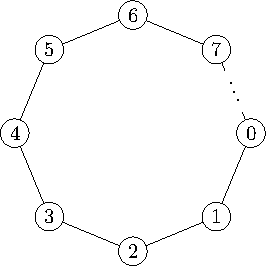
\includegraphics[width = 5cm]{cyclic_graph.pdf}
    \end{center}
    \item \textbf{Hypercube $Q_n$:} The $n$-dimensional Boolean hypercube is the Cayley graph of the group $(\mathbb{Z}_2)^n$ with generating set $S = \{e_1, \dots, e_n\}$, where $e_i$ flips the $i$-th bit. This graph is $n$-regular and bipartite.

    \item \textbf{Complete Graph $K_N$:} The complete graph on $N$ vertices can be viewed as the Cayley graph of $\mathbb{Z}_N$ with generating set $S = \{1, 2, \dots, N-1\}$ (all nonzero elements). Each vertex $g$ has an edge to every other vertex $g+s$.

    \item \textbf{Infinite Tree (Free Group):} The free group on two generators $a$ and $b$ has a Cayley graph that is an infinite 4-regular tree. Each vertex corresponds to a word in $\{a^{\pm1}, b^{\pm1}\}$, and edges represent multiplication by $a$ or $b$.

    \item \textbf{Dihedral Groups:} Cayley graphs of dihedral groups often form cyclic or prism-like structures. These graphs are used in modeling symmetric structures in both classical and quantum settings.
\end{itemize}

\subsection{Symmetry and Group Action}

Cayley graphs are highly symmetric. The group $G$ acts regularly on the vertices of $\Gamma(G, S)$ via left multiplication:
\[
g : h \mapsto gh.
\]
This action is:
\begin{itemize}
    \item \textbf{Vertex-transitive:} All vertices are structurally identical; there is no distinguished origin unless one is chosen explicitly.
    \item \textbf{Regular:} For any two vertices $u, v \in G$, there exists exactly one $g \in G$ such that $g \cdot u = v$.
\end{itemize}

This symmetry implies that quantum (or classical) walks can often be analyzed by considering representative initial conditions—commonly, the walk is assumed to start at the identity element $e$.

\subsection{Remarks}

Cayley graphs provide a powerful framework for analyzing quantum walks. Their regularity and symmetry often lead to analytical tractability, particularly using representation theory and spectral techniques. Throughout this thesis, we will explore quantum walks on Cayley graphs, leveraging their symmetry to obtain insights into walk dynamics and algorithmic applications.







\section{Quantum Walks on Cayley Graphs}


Cayley graphs provide an ideal setting for quantum walks due to their rich symmetry properties, which can be exploited to simplify analysis and implementation. Both continuous-time and discrete-time quantum walks on Cayley graphs have been studied extensively. We now highlight several key features and advantages of quantum walks in this setting.


%%%%%%%%%%%%%%%%%%%%%%%%%%%%%%%%%%%%%%%%%%%%%%%%%%%%%%%
\subsection{Spectral Structure}

The adjacency matrix $A$ of a Cayley graph is closely related to the group algebra of $G$. It can be expressed as:
\[
A = \sum_{a \in G} \lambda_a |\hat{a}\rangle \langle \hat{a}|,
\]
where $|\hat{a}\rangle$ is the quantum Fourier transform of $|a\rangle$. The eigenvalues $\lambda$ are given by
\[
\lambda_a = \sum_{q \in Q} \chi(a, q).
\]
Note that the eigenvectors $|\hat{a}\rangle$ of $A$ depend only on $G$ and not on the set $Q$.

To see this, we have

        \begin{align}
            A\ket{\hat{a}} 
            &= A\frac{1}{\sqrt{|G|}}\sum_{y \in G}\chi(a,y)\ket{y} \nonumber \\
            &= \frac{1}{\sqrt{|G|}}\sum_{y \in G}\chi(a,y)A\ket{y} \nonumber \\
            &= \frac{1}{\sqrt{|G|}}\sum_{y \in G}\chi(a,y)\sum_{q \in Q}\ket{qy} \nonumber
            \end{align}
            
            \noindent Consider $\beta = qy$. Then the above equation becomes:
            
            \begin{align}
            \frac{1}{\sqrt{|G|}}\sum_{q \in Q} \sum_{y \in G} \chi(a,y)\ket{qy} 
            &= \frac{1}{\sqrt{|G|}}\sum_{q \in Q} \chi(a,q) \sum_{\beta \in G} \chi(a,\beta)\ket{\beta} \nonumber \\
            &= \sum_{q \in Q} \chi(a,q)\ket{\hat{a}} \nonumber \\
            &= \lambda_a\ket{\hat{a}} \label{eq:group_action_walk}
            \end{align}
            


%%%%%%%%%%%%%%%%%%%%%%%%%%%%%%%%%%%%%%%%%%%%%%%%%%%%
\subsection{Structure and Symmetry in Cayley Graph Walks}

Cayley graphs possess vertex-transitive symmetry under the group action $g : h \mapsto gh$. This symmetry induces invariant subspaces for the quantum walk evolution. If the initial state is uniform over a symmetry orbit, it remains so under the walk.

In particular, for a continuous-time quantum walk starting at the identity element:
\[
\ket{\psi(t)} = e^{-iAt} \ket{e},
\]
the resulting state remains a \emph{class function}, i.e., the amplitude $\braket{g}{\psi(t)}$ depends only on structural properties of $g$ (such as Hamming weight or conjugacy class).

This symmetry drastically reduces the effective state space. For instance, on distance-regular graphs (including many Cayley graphs), amplitudes are equal for all vertices at the same distance from the starting point. This idea is also used in the analysis of the glued trees graph, where the walk remains uniform on each layer.


\paragraph{Discrete-Time Walks and Symmetry}
Coined DTQWs also benefit from Cayley graph symmetry. If a symmetric coin (e.g., the Grover coin) is used at each vertex of a vertex-transitive graph, the walk respects the full symmetry. As a result:
\begin{itemize}
    \item Amplitudes often remain uniform on symmetry-equivalent vertices.
    \item The dynamics of the walk can often be simplified by restricting to a smaller symmetric subspace.
    \item In some cases, symmetry can lead to localization, where amplitude becomes trapped due to spectral properties of the coin.
\end{itemize}
These effects can be mitigated or exploited through careful coin design or by using Szegedy’s method, which naturally respects symmetry.

In summary, Cayley graphs provide a rich and algebraically structured setting for quantum walks. Their underlying group-theoretic properties enable powerful techniques such as spectral analysis through irreducible representations, dimensionality reduction via symmetries and invariant subspaces, and explicit calculations of probabilities, mixing behavior, and hitting times. These features make Cayley graphs especially amenable to efficient quantum walk algorithms, which often exploit such structures either explicitly or implicitly. In the sections that follow, we extend these ideas to more general settings where group actions go beyond the framework of simple Cayley graphs.




\section{Cayley Graphs with Group Action}


Cayley graphs can also be generalized through group actions. Let \( (G, X, *) \) be a regular group action with a fixed element \( x \in X \), and let \( Q = \{q_1, q_2, \dots, q_k\} \subset G \) be a subset as before. Define the Cayley graph \( \Gamma = (X, E) \), where the vertex set is \( X \), and the edge set consists of all pairs \( (x, y) \in X \times X \) such that \( y = q * x \) for some \( q \in Q \).

The adjacency matrix of this graph can be written as:
\[
A = \sum_{h \in G} \lambda_h \ket{G^{(h)} * x} \bra{G^{(h)} * x},
\]
where
\[
\lambda_h = \sum_{q \in Q} \chi(h, q), \quad \text{and} \quad \ket{G^{(h)} * x} = \frac{1}{\sqrt{|G|}} \sum_{g \in G} \chi(g, h) \ket{g * x}.
\]

As in the previous case, the eigenvectors \( \ket{G^{(h)} * x} \) are determined solely by the structure of the group \( G \). This construction generalizes the standard Cayley graph: setting \( X = G \) and the group action \( * \) as group multiplication recovers the original definition.


Now, to see why we have the above equation, we have:



\begin{align}
    A\ket{G^{(h)} * x} 
    &= \frac{1}{\sqrt{|G|}}\sum_{g \in G} \chi(g, h)\, A\ket{g * x} \nonumber \\
    &= \frac{1}{\sqrt{|G|}}\sum_{g \in G} \chi(g, h)\sum_{q \in Q} \ket{q * (g * x)} \nonumber
    \end{align}
    
    \noindent Consider $\beta = qg$. Then the above equation becomes:
    
    \begin{align}
    \frac{1}{\sqrt{|G|}}\sum_{q \in Q} \sum_{\beta \in G} \chi(\beta, h)\chi(q, h)\ket{\beta * x}
    &= \sum_{q \in Q} \chi(q, h)\ket{G^{(h)} * x} \nonumber \\
    &= \lambda_h \ket{G^{(h)} * x} \label{eq:group_action_symmetrized}
    \end{align}

    Since the group action \( (G, X, *) \) is regular, the two Cayley graph constructions are isomorphic. In the first construction, the vertex set is \( G \), and the adjacency matrix is indexed by elements of \( G \). In the second construction, the vertex set is \( X \), with the adjacency matrix indexed by elements of \( X \). The isomorphism between these graphs is given by the bijection
\[
\setlength{\arraycolsep}{1mm}
\begin{array}{rcll}
\phi: & G & \longrightarrow & X \\
      & g & \longmapsto     & g * x,
\end{array}
\]

which maps each group element \( g \in G \) to the corresponding point in its orbit under the action.


    % Assuming the group action is a cryptographic group action, the isomorphism $\phi$ is a one-way function: given $g \in G$, it is easy to compute $g * x$, whereas given $(x, g * x)$, it is hard to compute $g$. Therefore, although these graphs are mathematically the same, computational problems based on them require fundamentally different techniques. A notable example is the implementation of quantum walks on these graphs.\footnote{Implementations of continuous-time quantum walks in the context of cryptographic group actions have previously appeared in \cite{booher2024failing, doliskani2023sample}, in the setting of supersingular isogeny graphs. These walks can be interpreted as group-action walks.} From this point onward, assume $Q$ is a small set, i.e., $\abs{Q} = \poly(\log \abs{G})$. In the first graph, we can efficiently implement the walks $e^{-iAt}$ even for values of $t$ that are exponentially large in $\log \abs{G}$. This follows from the fact that
    % \begin{equation}
    %     \label{eq:adjmat-fb}
    %     e^{-iAt} = \qft_G \sum_{a \in G} e^{-i\lambda_a t} \ket{a} \bra{a} \qft_G^*.
    % \end{equation}
    % The quantum Fourier transform $\qft_G$ and its inverse can be applied in $\poly(\log \abs{G})$ operations. The diagonal unitary in the middle, which is a phase computation $\ket{a} \mapsto e^{-i\lambda_a t} \ket{a}$, is also efficient because $\lambda_a$ can be computed classically to arbitrary precision in $\poly(\log \abs{G})$ time.
    
    % The situation for group actions is less straightforward. While the states $\ket{G^{(h)} * x}$ are analogous to the states $\ket{\hat{h}}$, the involvement of the action $*$ in the former introduces computational challenges. Specifically, it becomes hard to apply transformations beyond the action $\ket{y} \mapsto \ket{a * y}$ for $a \in G$. Consequently, no decomposition analogous to \eqref{eq:adjmat-fb} exists in the context of group actions. Instead, we are left with the spectral expression
    % \[ e^{-iAt} = \sum_{h \in G} e^{-i\lambda_h t} \ket{G^{(h)} * x} \bra{G^{(h)} * x}. \]
    % Despite this limitation, the sparsity and structure of the matrix $A$ allow us to demonstrate in the next section that for $t = \poly(\log \abs{G})$, the walk $e^{-iAt}$ can still be efficiently approximated to polynomial accuracy.   


    When the group action \( (G, X, *) \) is assumed to be cryptographic, the isomorphism \( \phi \) becomes a one-way function: given \( g \in G \), it is efficient to compute \( g * x \), but given the pair \( (x, g * x) \), it is computationally hard to recover \( g \). As a result, while the two Cayley graphs are mathematically isomorphic, computational tasks associated with them may require fundamentally different approaches. A particularly illustrative example is the implementation of quantum walks on these graphs.\footnote{Continuous-time quantum walks have been explored in the context of cryptographic group actions in~\cite{booher2024failing, doliskani2023sample}, specifically in supersingular isogeny graphs. These walks can be viewed as group-action quantum walks.}



% The concept of a Cayley graph generalizes naturally to the case of a group acting on an arbitrary set. Suppose a group $G$ acts transitively on a set $X$, and let $S \subset G$ be a generating set. We can construct a graph, often referred to as a \textbf{Schreier graph}, denoted $\Gamma(X; G, S)$, as follows:
% \begin{itemize}
%     \item The vertex set is $X$.
%     \item For each $x \in X$ and each $s \in S$, there is an edge from $x$ to $s \cdot x$.
% \end{itemize}

% This graph encodes the action of $G$ on $X$ and generalizes the Cayley graph construction. In fact, when $X \cong G/H$ for some stabilizer subgroup $H$ of a basepoint $x_0$, we interpret $\Gamma(X; G, S)$ as the \emph{Cayley graph of $G$ acting on the coset space $G/H$}. If $H$ is trivial (i.e., the action is regular), then $X \cong G$ and $\Gamma(X; G, S)$ reduces to the standard Cayley graph $\Gamma(G, S)$.

% When $H$ is nontrivial, several group elements from $G$ may correspond to the same vertex in $X$. Nonetheless, $\Gamma(X; G, S)$ inherits considerable symmetry from the group action:
% \begin{itemize}
%     \item $G$ acts by automorphisms on the graph,
%     \item The local structure of the graph is uniform across orbits.
% \end{itemize}

% \subsection{Examples}

% \begin{itemize}
%     \item \textbf{Symmetric group:} Let $G = S_n$ act on $X = \{1, \dots, n\}$ by permutations, and let $S$ be a generating set of transpositions. Then $\Gamma(X; G, S)$ is a complete graph on $n$ vertices, as any element can be swapped with any other via some $s \in S$.

%     \item \textbf{Johnson graphs:} These are Schreier graphs of $S_n$ acting on $k$-element subsets of $\{1, \dots, n\}$. Generators correspond to transpositions that change one element of the subset. Johnson graphs are highly symmetric and distance-regular, and they appear frequently in quantum walk algorithms.
% \end{itemize}

% \subsection{Quantum Walks on Group Action Graphs}

% Quantum walks on graphs arising from group actions share many of the useful features of walks on full Cayley graphs. In fact, one can often analyze a walk on $\Gamma(X; G, S)$ by \emph{lifting} it to a walk on the Cayley graph $\Gamma(G, S)$ and projecting down via the quotient map $G \to G/H$. This structure preserves symmetry in the transition amplitudes.

% In particular, if the initial quantum state is uniform over an orbit of $H$, the state will remain symmetric under the subgroup $H$ throughout the evolution. Thus, the walk evolves in an \emph{invariant subspace}, reducing the effective size of the problem.

% \textbf{Example – Quotient Walks:} Krovi and Brun (2007) analyzed quantum walks on quotient graphs and showed how hitting probabilities and mixing behavior can be improved by exploiting such symmetry reductions.

% Group action graphs are particularly useful in algorithmic settings where the state space is naturally modeled as an orbit under a group of moves or transformations. For instance:
% \begin{itemize}
%     \item The Rubik's cube configuration space is essentially the Cayley graph of the Rubik’s group acting on itself. Each configuration corresponds to a group element.
%     \item A quantum walk on this space is a specialized form of group action walk, where subgroups preserving partial configurations can be used to reduce search complexity.
% \end{itemize}

% \subsection{Summary}

% Graphs defined from group actions—such as Schreier graphs $\Gamma(X; G, S)$—generalize Cayley graphs to settings where the vertex set is a homogeneous space $G/H$. These graphs:
% \begin{itemize}
%     \item Maintain significant symmetry,
%     \item Enable reduction to invariant subspaces via subgroup structure,
%     \item Retain many spectral and dynamical properties of Cayley graphs.
% \end{itemize}

% Quantum walks on such graphs behave similarly to those on full Cayley graphs, though with potentially fewer vertices due to coset identification. This perspective is powerful for analyzing and implementing quantum algorithms.

In the next section, we develop techniques for simulating continuous-time quantum walks on such symmetric graphs using quantum circuits. These simulations exploit the group action structure to simplify circuit construction and enhance algorithmic efficiency.




\chapter{Simulating Group Action Quantum Walks}\label{chap:simulating}


From this point onward, we assume that the generating set \( Q \) is small, specifically \( \abs{Q} = \operatorname{poly}(\log \abs{G}) \). In the first construction, where the vertex set is \( X = G \), the continuous-time walk \( e^{-iAt} \) can be implemented efficiently even for values of \( t \) that are exponentially large in \( \log \abs{G} \). This efficiency stems from the identity:
\begin{equation}
    \label{eq:adjmat-fb}
    e^{-iAt} = \qft_G \left( \sum_{a \in G} e^{-i\lambda_a t} \ket{a} \bra{a} \right) \qft_G^*,
\end{equation}
where both \( \qft_G \) and its inverse can be implemented in \( \operatorname{poly}(\log \abs{G}) \) time. Moreover, the diagonal unitary \( \ket{a} \mapsto e^{-i\lambda_a t} \ket{a} \) is efficiently realizable since the eigenvalues \( \lambda_a \) can be computed classically to arbitrary precision in polynomial time with respect to \( \log \abs{G} \).

The situation becomes more nuanced in the group-action setting. Although the states \( \ket{G^{(h)} * x} \) play a role analogous to the Fourier basis states \( \ket{\hat{h}} \), the involvement of the group action \( * \) introduces additional complexity. In particular, implementing arbitrary transformations over these states is nontrivial. One is typically restricted to operations of the form \( \ket{y} \mapsto \ket{a * y} \), where \( a \in G \). Consequently, no efficient decomposition analogous to~\eqref{eq:adjmat-fb} is currently known in the group-action context. The best available formulation is the spectral decomposition:
\[
e^{-iAt} = \sum_{h \in G} e^{-i\lambda_h t} \ket{G^{(h)} * x} \bra{G^{(h)} * x}.
\]

Despite these challenges, the adjacency matrix \( A \) still exhibits substantial sparsity and algebraic structure. In the following section, we demonstrate that for \( t = \operatorname{poly}(\log \abs{G}) \), the walk \( e^{-iAt} \) remains efficiently approximable to polynomial accuracy.


%%%%%%%%%%%%%%%%%%%%%%%%%%%%%%%%%%%%%%%%%%%%%%%%%%%%%%%


\section{Simulating continuous-time walks}
Childs~\cite{Childs2004}, Berry and Kothari~\cite{BerryKothari} showed that continuous-time quantum walks can be simulated using discrete-time quantum walks. Since our approach relies on their methods, we begin by outlining the relevant notation and framework.

Let \( H \) be a Hamiltonian of dimension \( N = 2^n \), and define \( \opnorm{H}_{\mathrm{max}} = \max_{i, j} \abs{H_{ij}} \). To facilitate the simulation, we expand the Hilbert space from \( \mathbb{C}^N \) to \( \mathbb{C}^{2N} \otimes \mathbb{C}^{2N} \) by appending an ancilla qubit initialized to \( \ket{0} \) and duplicating the resulting space.

To define the discrete-time walk operator, we first construct an orthonormal set of states:
\begin{align}
    \ket{\phi_{j0}} & := \frac{1}{\sqrt{d}} \sum_{\ell \in F_j} \ket{\ell} \left( \sqrt{\frac{H_{j\ell}^*}{K}} \ket{0} + \sqrt{1 - \frac{\abs{H_{j\ell}^*}}{K}} \ket{1} \right), \label{eq:walk-sim} \\
    \ket{\phi_{j1}} & := \ket{0} \ket{1}, \nonumber
\end{align}
where \( F_j \) denotes the set of nonzero entries in column \( j \) of \( H \), and \( K \ge \opnorm{H}_{\mathrm{max}} \) is a fixed constant.

Based on these states, we define the isometry \( T : \C^{2N} \to \mathbb{C}^{2N} \otimes \mathbb{C}^{2N} \) as follows:
\begin{equation}
    \label{eq:walk-isom}
    T := \sum_{j = 0}^{N - 1} \sum_{b \in \{0, 1\}} (\ket{j}\bra{j} \otimes \ket{b}\bra{b}) \otimes \ket{\phi_{jb}}.
\end{equation}

The discrete-time quantum walk operator is then defined as
\[
W = iS(2TT^* - \mathds{1}),
\]
where \( S \) is the swap operator acting as
\[
S \ket{j_1} \ket{b_1} \ket{j_2} \ket{b_2} = \ket{j_2} \ket{b_2} \ket{j_1} \ket{b_1},
\]
for all \( 0 \le j_1, j_2 < N \) and \( b_1, b_2 \in \{0, 1\} \).

To efficiently simulate the continuous-time evolution \( e^{-iHt} \), it suffices to implement the isometry \( T \), its adjoint \( T^* \), and the walk operator \( W \) efficiently.
%  Assuming black-box (oracle) access to the entries of \( H \), the following result holds:

% \begin{theorem}[{\cite[Theorem 1]{berry2015hamiltonian}}]
% \label{thm:sparse-sim}
% Let \( H \) be a \( d \)-sparse Hamiltonian acting on \( n \) qubits. Then the unitary \( e^{-iHt} \) can be approximated to within error \( \epsilon \) using
% \[
% O\left( \tau \frac{\log(\tau / \epsilon)}{\log\log(\tau / \epsilon)} \right)
% \]
% queries to \( H \), and
% \[
% O\left( \tau \left[ n + \log^{5 / 2}(\tau / \epsilon) \right] \frac{\log(\tau / \epsilon)}{\log\log(\tau / \epsilon)} \right)
% \]
% additional elementary gates, where \( \tau = d \cdot \opnorm{H}_{\mathrm{max}} \cdot t \).
% \end{theorem}







\section{Simulating group action quantum walks.}
Assume \( t = \operatorname{poly}(\log \abs{G}) \). We show that the continuous-time walk \( W = e^{-iAt} \) can be efficiently simulated using the discrete-time quantum walk framework developed in~\cite{childs2010relationship}. Recall the isometry \( T \) defined in Equation~\eqref{eq:walk-isom}, where the states \( \ket{\phi_b} \) are as given in Equation~\eqref{eq:walk-sim}. To carry out the simulation, it suffices to show that the isometry \( T \), its adjoint \( T^* \), and the discrete-time walk operator
\[
W = iS(2TT^* - \mathds{1})
\]
can all be efficiently implemented in the group-action setting.


Let \( \Gamma = (X, E) \) be the Cayley graph associated with the group action \( (G, X, *) \), and let \( A \) denote its adjacency matrix. The Hamiltonian \( H \) of interest is simply \( A \), indexed by elements of \( X \). In this context, the isometry \( T \) takes the form:
\begin{align*}
T
& := \sum_{y \in X} \sum_{b \in \{0, 1\}} (\ket{y}\bra{y} \otimes \ket{b}\bra{b}) \otimes \ket{\phi_{yb}} \\
& = \sum_{y \in X} \sum_{b \in \{0, 1\}} \ket{y} \ket{b} \ket{\phi_{yb}} \bra{y} \bra{b}.
\end{align*}


Because of the structure of $\Gamma$, the states \eqref{eq:walk-sim} simplify as follows. First, since the set $Q$ is symmetric, the graph $\Gamma$ is undirected and the adjacency matrix $A$ is symmetric with non-negative entries; the nonzero entries of $A$ are all equal to $1$. Therefore, we can set $K = \opnorm{A}_{\mathrm{max}} = 1$. As a result, for $y \in X$, the state $\ket{\phi_{y0}}$ becomes
\[ \ket{\phi_{y0}} = \frac{1}{\sqrt{\abs{Q}}} \sum_{q \in Q} \ket{q * y} \ket{0}. \]
We now describe how to implement the isometry \( T \) by constructing efficient unitaries \( U_0 \) and \( U_1 \), where each \( U_b \) acts as
\[
U_b : \ket{0} \ket{y, b} \ket{0, 0} \mapsto \ket{0} \ket{y, b} \ket{\phi_{yb}}, \quad b \in \{0, 1\},
\]
with the first register serving as an ancilla.

The unitary \( U_1 \) is straightforward to implement, since \( \ket{\phi_{y1}} = \ket{0} \ket{1} \) is independent of \( y \). We now focus on the construction of \( U_0 \).

Because \( Q \subset G \) is a small set (i.e., \( \abs{Q} = \operatorname{poly}(\log \abs{G}) \)), we can construct an efficient unitary \( V_Q : \mathbb{C}^Q \to \mathbb{C}^Q \) such that
\[
V_Q \ket{0} = \frac{1}{\sqrt{\abs{Q}}} \sum_{q \in Q} \ket{q}.
\]
Applying \( V_Q \otimes \mathds{1} \) to the state \( \ket{0} \ket{y, 0} \ket{0, 0} \) produces:
\[
\frac{1}{\sqrt{\abs{Q}}} \sum_{q \in Q} \ket{q} \ket{y, 0} \ket{0, 0}.
\]

Next, we apply the unitary \( V_1 \), defined by:
\[
V_1 : \ket{q} \ket{y, 0} \ket{0, 0} \mapsto \ket{q} \ket{y, 0} \ket{q * y, 0}.
\]

Following this, we uncompute the first register to recover \( \ket{0} \ket{y, 0} \ket{\phi_{y0}} \). This is achieved by applying the unitary \( V_2 \), defined as:
\[
V_2 : \ket{q} \ket{y, 0} \ket{q * y, 0} \mapsto \ket{0} \ket{y, 0} \ket{q * y, 0}.
\]
Since \( Q \) is small, we can efficiently determine \( q \) from the pair \( (y, q * y) \) by exhaustively checking each \( q \in Q \). Thus, \( V_2 \) (and therefore \( U_0 \)) can be implemented efficiently.


To implement \( U_0^* : \ket{0} \ket{y, 0} \ket{\phi_{y0}} \mapsto \ket{0} \ket{y, 0} \ket{0, 0} \), we sequentially apply \( V_2^* \), followed by \( V_1^* \), and finally \( V_Q^* \otimes \mathds{1} \). Since each of these unitaries can be implemented efficiently, it follows that \( U_0^* \) is also efficient.

We now construct the isometry \( T \) using a conditional unitary \( U_T \), which applies either \( U_0 \) or \( U_1 \) depending on the value of the qubit \( b \). That is,
\[
U_T = \text{Controlled-}U_b \quad \text{with control on } b \in \{0,1\}.
\]

Next, we demonstrate that the walk unitary
\[
W = iS(2TT^* - \mathds{1})
\]
can be applied efficiently. This reduces to implementing the reflection \( 2TT^* - \mathds{1} \), which we analyze as follows:
\begin{align*}
2\ket{0}\bra{0} \otimes TT^* - \mathds{1}
&= 2\ket{0}\bra{0} \otimes \sum_{y \in X} \sum_{b \in \{0,1\}} \ket{y,b} \ket{\phi_{yb}} \bra{y,b} \bra{\phi_{yb}} - \mathds{1} \\
&= 2\sum_{y \in X} \sum_{b \in \{0,1\}} \ket{0} \ket{y,b} \ket{\phi_{yb}} \bra{0} \bra{y,b} \bra{\phi_{yb}} - \mathds{1} \\
&= U_T \left( 2 \sum_{y \in X} \sum_{b \in \{0,1\}} \ket{0} \ket{y,b} \ket{0,0} \bra{0} \bra{y,b} \bra{0,0} - \mathds{1} \right) U_T^* \\
&= U_T \left( 2\ket{0}\bra{0} \otimes \mathds{1}_{X,b} \otimes \ket{0,0}\bra{0,0} - \mathds{1} \right) U_T^*.
\end{align*}

Since \( U_T \), \( U_T^* \), and the operator \( 2\ket{0}\bra{0} \otimes \mathds{1}_{X,b} \otimes \ket{0,0}\bra{0,0} - \mathds{1} \) can all be implemented efficiently, it follows that the reflection \( 2\ket{0}\bra{0} \otimes TT^* - \mathds{1} \) is also efficient.

Finally, for any input state \( \ket{\psi} \), the reflection acts as:
\[
\left(2\ket{0}\bra{0} \otimes TT^* - \mathds{1} \right) \ket{0} \ket{\psi} = \ket{0} \left(2TT^* - \mathds{1} \right) \ket{\psi},
\]
confirming that the full walk operator \( W \) can be implemented efficiently in the group-action setting.





% \section{Hamiltonian Structure and Sparsity}

% \section{Quantum Walk-Based and QSP Simulation}

% \section{Complexity Analysis}




\chapter{Quantum Money and Hartley Transform}\label{chap:quantum_money}

We now present our public-key quantum money scheme based on group actions and the Hartley transform. We begin by reviewing Zhandry’s quantum money scheme from abelian group actions (which uses the Fourier transform) as a baseline. Then we describe our Hartley-transform-based variant and discuss its properties. The quantum Hartley transform will play a central role in both the generation and verification of banknotes.

\section{Public-Key Quantum Money: Definitions}
A public-key quantum money scheme consists of two algorithms, traditionally called $\mathsf{Gen}$ and $\mathsf{Verify}$:
\begin{itemize}
    \item $\mathsf{Gen}(1^n)$ is a probabilistic quantum polynomial-time (QPT) algorithm that, given a security parameter $n$, outputs a pair $(s, |\$\rangle)$. Here $s$ is a classical string called the \emph{serial number} (or public key) and $|\$\rangle$ is a quantum state representing the banknote. We often call the pair $(s, |\$\rangle)$ a banknote, and $s$ by itself the serial number of that banknote.
    \item $\mathsf{Verify}(s, |\$\rangle)$ is a QPT algorithm (which may be implemented as a quantum circuit acting on the state $|\$\rangle$ and some ancillary workspace). It takes as input a serial number $s$ and an alleged quantum banknote state $|\$\rangle$. It outputs $\mathtt{accept}$ (valid) or $\mathtt{reject}$ (invalid).
\end{itemize}

We require two properties from such a scheme:
\begin{description}
    \item[Correctness:] For any valid output $(s, |\$\rangle)$ of $\mathsf{Gen}(1^n)$, the verification algorithm accepts with high probability. Formally, $\Pr[\mathsf{Verify}(s, |\$\rangle) = \mathtt{accept}]$ should be very close to 1 (typically we require it to be $1 - \negl(n)$, where $\negl(n)$ denotes a negligible function in $n$).
    \item[Security (Unforgeability):] No efficient adversary, given one or more genuine banknotes, can produce a new valid banknote. In the strongest formulation, if an adversary is given a single valid $(s, |\$\rangle)$, it should be infeasible for them to produce two quantum states $|\$'\rangle$ and $|\$''\rangle$ such that $\mathsf{Verify}(s, |\$'\rangle) = \mathsf{Verify}(s, |\$''\rangle) = \mathtt{accept}$ (i.e., they cannot create a second copy that passes verification while retaining the original). More generally, even given multiple banknotes, the adversary should not be able to create new ones with fresh serial numbers that pass verification. This captures the idea that quantum money cannot be counterfeited.
\end{description}

In a \emph{public-key} scheme, the verifier uses only the public information (here, the serial number and any scheme-wide public parameters) to check validity, and does not need any secret key. The bank may have a secret key to produce the states, but after generation, the bank’s involvement is not needed. In our scheme, the serial number will effectively contain the information needed for public verification (similar to how a classical bill might have a number anyone can look up, except here it’s used in a quantum procedure).

We next outline Zhandry’s scheme, which our scheme builds upon.

\section{Fourier-Based Quantum Money from Group Actions}
Zhandry’s quantum money scheme \cite{Zhandry2024} is built on an abelian group action $*:G \times X \mapsto X$. We have a family of group actions parameterized by the security parameter $n$ (so the size of $G$ grows with $n$). For simplicity, assume $|G| = N$. The scheme also fixes a particular element $x_0 \in X$ that everyone knows (a public base point in $X$).

The generation algorithm $\mathsf{Gen}$ in Zhandry’s scheme works as follows (informally):
\begin{enumerate}
    \item On input $1^n$, sample a random group element $h \leftarrow G$. This $h$ will serve as the serial number $s$ for the banknote.
    \item Prepare two registers: the first is a group element register, initialized to $|0_G\rangle$ (an encoding of the identity element of $G$), and the second is an $X$-register initialized to $|x_0\rangle$.
    \item Apply the quantum Fourier transform over $G$ to the first register. This creates a uniform superposition over $G$: 
    \[
    \frac{1}{\sqrt{N}} \sum_{g \in G} |g\rangle \otimes |x_0\rangle\,.
    \] 
    \item Now apply the group action in a controlled manner: for each basis state $|g\rangle$ in the first register, apply $g$’s action on the second register. This transforms the joint state into 
    \[
    \frac{1}{\sqrt{N}} \sum_{g \in G} |g\rangle \otimes |g * x_0\rangle\,,
    \] 
    which is an entangled state between a superposition of group elements and their corresponding $X$-elements.
    \item Apply the inverse $\qft$ (which is the adjoint of the $\qft$) on the first register. This recombines the amplitudes in the first register. The result (by properties of the $\qft$) can be shown to be 
    \[
    \frac{1}{\sqrt{N}} \sum_{g \in G} \omega^{\langle h,\,g \rangle} |g\rangle \otimes |g * x_0\rangle\,,
    \] 
    where $\omega^{\langle h,\,g \rangle}$ denotes the phase picked up that depends on $h$ and $g$. In fact, this state can be written as $|h\rangle \otimes \frac{1}{\sqrt{N}}\sum_{g \in G} |g * x_0\rangle$; essentially, the first register ends up in $|h\rangle$ (the serial number) and the second register is an equal superposition of all elements of $X$ in the orbit of $x_0$ (which is $X$ itself, since the action is transitive) but weighted by a phase related to $h$. This is the so-called group-action Fourier state.
    \item The first register (which contains $|h\rangle$) is measured in the computational basis, yielding the random serial number $g$ and collapsing the second register to a state that we will denote $|\$_h\rangle$. This $|\$_h\rangle$ is the actual quantum money state corresponding to serial $h$.
    \item Output the pair $(s = h,\; |\$\rangle = |\$_h\rangle)$.
\end{enumerate}

In the above, a bit of algebra reveals that $|\$_h\rangle = \frac{1}{\sqrt{N}} \sum_{g\in G} \chi(h,g)\, |g * x_0\rangle$, where $\chi(h,g) = \omega^{\langle h,\,g \rangle}$ is essentially the character of $G$ indexed by $h$. In other words, $|\$_h\rangle$ is (up to global phase) the state one gets by applying the representation (character) $\chi(h,.)$ to weight the superposition over the orbit $X$. These states for different $h$ are almost orthogonal and can be distinguished with the right measurement.

The verification algorithm $\mathsf{Verify}(h, |\$_h\rangle)$ for Zhandry’s scheme goes as follows:
\begin{enumerate}
    \item Given the purported serial number $h \in G$ and an input state $|\psi\rangle$ (which should equal $|\$_h\rangle$ if genuine), attach an auxiliary register prepared in $|x_0\rangle$.
    \item Perform a controlled group action “kickback” using $h$ on the auxiliary register. Specifically, perform the unitary that maps $|y\rangle \otimes |x_0\rangle \mapsto |y\rangle \otimes |h * x_0 \rangle$ for each basis element $|y\rangle$ of the first register. (This operation uses the classical $h$ to act on the second register conditioned on the first—essentially, it multiplies the second register’s state by $h$ if the first register is in an appropriate basis state. There are various ways to implement this, but conceptually it’s a controlled operation using the known $h$.)
    \item Now measure the second register (the auxiliary one) in the computational basis of $X$ to see if it is still $|x_0\rangle$. If the state $|\psi\rangle$ was the correct Fourier state $|\$_h\rangle$, one can show that this measurement will yield $x_0$ with high probability (constructive interference causes the $x_0$ component to be strong). If $|\psi\rangle$ was not the correct state, the measurement is unlikely to give $x_0$.
    \item Accept if and only if the measurement outcome is $x_0$ (i.e. the second register returns to the base state).
\end{enumerate}

The intuition is that the genuine state $|\$_h\rangle$ contains a phase that exactly cancels out the action of $h$ in the verification step, causing the auxiliary register to end up back at $x_0$. A counterfeit state, by contrast, would not generally have the right phase relationship, and the auxiliary register’s state would be some superposition over $X$ that is not concentrated on $x_0$, hence likely giving a different outcome upon measurement.

Zhandry’s scheme is shown to be correct (valid notes pass) and is believed to be secure under the assumption that the group action is one-way. The hardness essentially boils down to: given $x_0$ and $|\$_h\rangle$, an adversary cannot figure out a different $h'$ that would produce a second valid state $|\$_{h'}\rangle$ or replicate $|\$_h\rangle$ (because that would solve the hidden subgroup or discrete log type problem in the group action).

\section{Hartley-Transform Money Scheme Construction}


Our scheme modifies the above Fourier-based construction by utilizing the \textbf{quantum Hartley transform ($\qht$)} in place of the $\qft$. Since the Hartley transform is closely related to the Fourier transform (essentially it produces the real and imaginary parts in a single real-valued transform), one might expect this substitution to be straightforward. And indeed, for the generation procedure it largely is: we will use the $\qht$ to create real-amplitude superposition states.

Concretely, assume again a group action $*: G\times X \mapsto X$ with $|G|=N$. For concreteness, we assume that $G = \Z_N$; the genralization of the scheme to a general group $G$ is straightforward. We fix the same generating set $S$ and basepoint $x_0$. The $\mathsf{Gen}_{H}$ (Hartley generation) algorithm:
\begin{enumerate}
    \item Sample a random $h \leftarrow G$ to be the serial number.
    \item Prepare $|0_G, x_0\rangle$ as before.
    \item Apply the \emph{quantum Hartley transform} over $G$ to the first register, as we saw in \ref{eq:qht-N}:
    \[
       \qht: |g\rangle \mapsto \frac{1}{\sqrt{N}} \sum_{k \in \mathbb{Z}_N} \cas \Big(\frac{2\pi  kg }{N}\Big) |k\rangle,
    \] 
    where $\mathrm{cas}(\theta) = \cos \theta + \sin \theta$. In simpler terms, $\qht(|0_G\rangle) = \frac{1}{\sqrt{N}}\sum_{k \in G} |k\rangle$ (because $\cas(0)=1$), \emph{the same uniform superposition as the $\qft$ produces for $|0\rangle$}. So after this step, we again have $\frac{1}{\sqrt{N}}\sum_{g \in G} |g\rangle|x_0\rangle$, but crucially the coefficients are all \emph{real} and positive (in fact all $1/\sqrt{N}$).
    \item Perform the controlled group action by the first register on the second: $\frac{1}{\sqrt{N}}\sum_{g} |g\rangle |g*x_0\rangle$.
    \item Apply the inverse $\qht$ on the first register (which being its own inverse up to a constant factor, is the same operation again since Hartley is symmetric like Fourier). Now here is where things differ: after this operation, the joint state will be 
    \[
       \frac{1}{\sqrt{N}} \sum_{g \in \mathbb{Z}_N} \cas\Big(\frac{2\pi hg}{N}\Big)\, |g\rangle \otimes |g*x_0\rangle.
    \] 
    Because the Hartley transform combines what would be cosine and sine terms, this state is not as nicely factorable as in the Fourier case. In the Fourier case, we got $|h\rangle \otimes \text{(orbit state)}$. In the Hartley case, we do not get a single basis state in the first register; instead we get a superposition in the first register with real coefficients $c_g = \cas(2\pi hg/N)$. However, note that $c_g$ is just some real number in $[-1,1]$ depending on $h$ and $g$. Another way to express the above state is:
    \[
      |\$\rangle = \frac{1}{\sqrt{N}} \sum_{x \in X} \Big(\frac{1}{\sqrt{N}}\sum_{g: g*x_0 = x} \cas\big(\frac{2\pi  hg}{N}\big)\Big)\, |x\rangle.
    \] 
    Since for a given $x\in X$, all $g$ such that $g*x_0=x$ have the form $g = u h$ for a unique $u \in G$ (because the action is free and transitive), one can simplify the internal sum using properties of the cas function. But we need not dive into that here.
    \item No measurement of the first register is performed. In fact, we do not have a nice product state separation, so we cannot simply measure one register to get $h$. Instead, the output of generation is just the quantum state $|\$\rangle$ (which is entangled between what used to be two registers) and the known classical serial number $h$ (we know what $h$ we picked).
\end{enumerate}

The resulting money state $|\$\rangle$ has only real amplitudes (because the initial superposition was real and the controlled operation doesn’t introduce complex numbers, and the Hartley transform yields real coefficients). In particular, in the computational basis of $X$, the state $|\$\rangle$ is some real-vector state (with both positive and negative values possible). We can think of it as a “Hartley orbit state” corresponding to $h$.

The verification algorithm in our Hartley-based scheme attempts to mirror the Fourier-based verification: it will use the given serial $h$ and try to check the state. A first idea would be: do exactly the same as Zhandry’s verify (the group-action kickback and measure). However, this fails in certain cases. Specifically, the Hartley transform being real causes an ambiguity: it turns out that there exist distinct $h \neq h'$ for which the Hartley-based states $|\$\rangle_h$ and $|\$\rangle_{h'}$ are not orthogonal, and the original verification might accept a forged state that is a certain superposition. In fact, the verification algorithm might accept an illegitimate state with some probability bounded away from zero. This is the “breakdown” of the straightforward Hartley substitution that we alluded to earlier.

To address this, our verification algorithm takes a more sophisticated approach:
\begin{enumerate}
    \item Given $(h, |\psi\rangle)$, it first uses the \textbf{quantum walk-based phase estimation} method (to be detailed in Chapter 6) to \emph{compute the eigenphase corresponding to $h$}. In short, we will treat $|\psi\rangle$ as an eigenvector of the group action adjacency matrix with a certain eigenvalue $\lambda$ related to $h$. We run a procedure to estimate $\lambda$ to high precision.
    \item From the estimated eigenvalue(s), we reconstruct a candidate group element $h^*$ that we believe generated the state. (This uses the fact that by running phase estimation for multiple carefully chosen walk durations, one can solve for $h$ as shown in \cite{Zhandry2022}.)
    \item We check if $h^* = h$ (the serial number provided). If not, we reject, since the state does not match the serial. If yes, we accept.
\end{enumerate}

This procedure essentially extracts the hidden group element from the state and compares it to the claimed serial. If an adversary tries to forge a state $|\psi\rangle$ for a known serial $h$, the only way to consistently pass verification is if $|\psi\rangle$ truly encodes the same $h$ in its eigen-spectrum. A fake note that was causing trouble for the naive Hartley verification (e.g., a state that is a mixture of two different “Hartley orbit” states) would yield an eigenphase that does not correspond to a single valid $h$, and the algorithm would detect the mismatch.

The key quantum tool enabling this verification is the continuous-time quantum walk on the group action graph and the ability to simulate it, which we prepared in Chapter 4. The walk Hamiltonian $A(X,S)$ has the genuine money state $|\$\rangle_h$ as an eigenstate with a known eigenvalue $\lambda(h)$. By running phase estimation on $e^{-iA t}$ with the state $|\psi\rangle$, we attempt to measure that eigenvalue. We repeat for a few different values of $t$ (the “twists” or different phases) to get enough information to pinpoint $h$. This approach can be viewed as adding extra “twists” to the verification: effectively, each choice of $t$ in phase estimation is like looking at the state in a different interference fringe pattern, analogous to applying different group actions as twists in the verification procedure. This is why we described the new verification as using group action twists—by varying a continuous parameter related to the group action’s eigenvalues, we break the symmetry that allowed a counterfeit to slip through.

We defer the full analysis of the success probabilities and how many repetitions are needed to Chapter 6, where we describe the verification algorithm in detail. For now, the takeaway is that by using the quantum walk approach, we can reliably verify Hartley-based money states, restoring security while still enjoying the properties of real amplitudes.

\section{Efficient Quantum Hartley Transform Implementation}\label{sec:efficient_qht}
Before moving on to the verification algorithm, we briefly discuss how we implement the quantum Hartley transform ($\qht$) efficiently, as this is an important practical aspect of our scheme. The Fourier transform is well-known to have efficient circuits; for the Hartley transform, fewer results are available, so we contributed a new circuit construction.

The $\qht$ we need is over an abelian group, which for concreteness one can think of as $\mathbb{Z}_N$ (the general finite abelian group case can usually be reduced to a direct sum of cyclic groups, applying $\qht$ on each cyclic component). Classical Hartley transforms have a recursive structure similar to fast Fourier transforms. In fact, there are known formulas to express a Hartley transform of size $N$ in terms of two Hartley transforms of size $N/2$ plus some additional linear operations \cite{Bracewell1984}. We leveraged such structures to design a divide-and-conquer quantum circuit.

Our algorithm for $\qht$ works roughly as follows:
- If $N$ is even, we can express the length-$N$ Hartley transform in terms of two length-$N/2$ Hartley transforms plus a combination of cheap operations (additions, permutations of data, etc.). We implement this decomposition recursively as a quantum circuit. The base of the recursion is when the size is small (like $N=2$ or $4$, where the transform can be done with a constant number of gates).
- We found that by carefully optimizing this recursion and using some known quantum subroutines for certain linear combinations, the overall gate count is improved compared to naive methods or previous proposals \cite{Klappenecker2001DCT,Klappenecker2001Signal}. In particular, our circuit avoids introducing any quantum Fourier transform internally (unlike \cite{Klappenecker2001Signal} which computed Hartley via Fourier plus some adjustments), and this yields a purely real rotation-based circuit.


%%%%%%%%%%% az inja %%%%%%%%%%%%%

Our algorithm for the quantum Hartley transform, \( \qht_N \), is modeled after the recursive structure of the quantum Fourier transform algorithm \( \qft_N \). To motivate this, we begin by reviewing the standard approach for computing \( \qft_N \). For clarity, we assume \( N = 2^n \), allowing each element of \( \mathbb{Z}_N \) to be represented using exactly \( n \) qubits. The same recursive framework can be extended to handle general values of \( N \). For any \( a \in \mathbb{Z}_N \), the quantum Fourier transform is defined as:


\begin{align}
    \qft_N\ket{a}
    & = \frac{1}{\sqrt{N}} \sum_{y = 0}^{N - 1} \omega_N^{ay}\ket{y} \\
    & = \frac{1}{\sqrt{N}} \sum_{y = 0}^{N / 2 - 1} \omega_N^{ay} \ket{y} + (-1)^a \frac{1}{\sqrt{N}} \sum_{y = 0}^{N / 2 - 1} \omega_N^{ay} \ket{y + N/2} \\
    & = \frac{1}{\sqrt{N / 2}} \sum_{y = 0}^{N / 2 - 1} \omega_N^{ay} \frac{1}{\sqrt{2}} (\ket{0} + (-1)^a \ket{1}) \ket{y}, \label{eq:qft_alt}
\end{align}


In the final expression, we have isolated the first qubit for clarity. Let \( \ket{a} = \ket{t}\ket{b} \), where \( b \) denotes the least significant bit of \( a \), implying that \( a = 2t + b \) for some \( t \in \mathbb{Z}_{N / 2} \). Applying \( \qft_{N / 2} \) to the first register yields the state:

\[ \frac{1}{\sqrt{N / 2}} \sum_{y = 0}^{N / 2 - 1} \omega_N^{2ty} \ket{y} \ket{b}. \]
Next, we apply the phase unitary \( P(y, b) \), defined by \( \ket{y} \ket{b} \mapsto \omega_N^{by} \ket{y} \ket{b} \), followed by a Hadamard transform on the final qubit. This results in the state given in Equation~\eqref{eq:qft_alt}.


We now describe our algorithm for efficiently computing the quantum Hartley transform \( \qht_N \). The key idea is to leverage the recursive structure of \( \qht_N \), analogous to the strategy used for \( \qft_N \). To facilitate this, we begin by rewriting the summation in Equation~\eqref{eq:qht-N} to expose its recursive form. Our approach is as follows:
\begin{equation}
    \label{eq:cas-expand}
	\frac{1}{\sqrt{N}} \sum_{y = 0}^{N - 1} \cas\Big( \frac{2\pi a y}{N} \Big) \ket{y}
    = \frac{1}{\sqrt{N}} \sum_{y = 0}^{N / 2 - 1} \cas\Big( \frac{2\pi a y}{N} \Big) \ket{y} + \frac{1}{\sqrt{N}} \sum_{y = N / 2}^{N - 1} \cas\Big( \frac{2\pi a y}{N} \Big) \ket{y}.
\end{equation}



The second summation on the right-hand side can be expressed as:
\begin{align*}
	\sum_{y = N / 2}^{N - 1} \cas\Big( \frac{2\pi a y}{N} \Big) \ket{y}
    & = \sum_{y = 0}^{N / 2 - 1} \cas\Big( \frac{2\pi a y}{N} + \pi a \Big) \ket{y + N/2} \\
    & = (-1)^a \sum_{y = 0}^{N / 2 - 1} \cas\Big( \frac{2\pi a y}{N} \Big) \ket{y + N/2},
\end{align*}
The second equality follows from the angle-sum identity for the \( \cas \) function,
\[
\cas(\alpha + \beta) = \cos(\alpha)\cas(\beta) + \sin(\alpha)\cas(-\beta),
\]
along with the fact that \( \cos(\pi a) = (-1)^a \) for all integers \( a \). Substituting this into Equation~\eqref{eq:cas-expand} yields:
\begin{align}
	\frac{1}{\sqrt{N}} \sum_{y = 0}^{N - 1} \cas\Big( \frac{2\pi a y}{N} \Big) \ket{y}
    & = \frac{1}{\sqrt{N}} \sum_{y = 0}^{N / 2 - 1} \cas\Big( \frac{2\pi a y}{N} \Big) (\ket{y} + (-1)^a \ket{y + N/2}) \nonumber \\
    & = \frac{1}{\sqrt{N / 2}} \sum_{y = 0}^{N / 2 - 1} \cas\Big( \frac{2\pi a y}{N} \Big) \frac{1}{\sqrt{2}} (\ket{0} + (-1)^a \ket{1}) \ket{y}, \label{eq:qht-alt} 
\end{align}
In the final equality, the most significant qubit has been isolated to emphasize its contribution to the overall transformation.

We now demonstrate how to compute \( \qht_N \) recursively. For a given \( a \in \mathbb{Z}_N \), we decompose the basis state as \( \ket{a} = \ket{t}\ket{b} \), where \( b \) denotes the least significant bit, such that \( a = 2t + b \) for some \( t \in \mathbb{Z}_{N/2} \). Assuming the existence of an efficient quantum circuit for computing \( \qht_{N/2} \), we proceed to construct \( \qht_N \) in a recursive fashion. To begin the transformation on \( \ket{a} \), we introduce an ancilla qubit initialized to \( \ket{0} \), yielding the joint state \( \ket{0}\ket{t}\ket{b} \). We then proceed as follows:
\begin{align*}
	\ket{0}\ket{t}\ket{b}
    & \mapsto \frac{1}{\sqrt{N / 2}} \sum_{y = 0}^{N / 2 - 1} \cas\Big( \frac{2\pi t y}{N / 2} \Big) \ket{0} \ket{y} \ket{b} & (\mathds{1} \otimes \qht_{N / 2} \otimes \mathds{1}) \\
    & = \frac{1}{\sqrt{N / 2}} \sum_{y = 0}^{N / 2 - 1} \cas\Big( \frac{4\pi t y}{N} \Big) \ket{0} \ket{y} \ket{b} \\
    & \mapsto \frac{1}{\sqrt{N}} \sum_{y = 0}^{N / 2 - 1} \cas\Big( \frac{4\pi t y}{N} \Big) (\ket{0} + \ket{1}) \ket{y}\ket{b}. & (H \otimes \mathds{1})
\end{align*}
Here, $\mathds{1} \otimes \qht_{N / 2} \otimes \mathds{1}$ is a unitary that applies the identity to the first and last qubits and applies $\qht_{N/2}$ to the rest of the qubits. Next, we apply a controlled negation operation, where the ancilla qubit is flipped if and only if the least significant bit \( b \) is equal to 1.
\[
    V: \ket{0}\ket{y} \mapsto \ket{0}\ket{y}, \quad \ket{1}\ket{y} \mapsto \ket{1}\ket{N / 2 -y},
\]
\[
    \frac{1}{\sqrt{N}} \sum_{y = 0}^{N / 2 - 1} \cas\Big( \frac{4\pi t y}{N} \Big) \ket{0} \ket{y} \ket{b} + \frac{1}{\sqrt{N}} \sum_{y = 0}^{N / 2 - 1} \cas\Big( \frac{4\pi t y}{N} \Big) \ket{1} \ket{-y} \ket{b}.
\]
By performing a change of variables in the second summation and using the identity \( \cas\left(\frac{4\pi t (N / 2 - y)}{N}\right) = \cas\left(-\frac{4\pi t y}{N}\right) \), we obtain the state:
\[
    \frac{1}{\sqrt{N}} \sum_{y = 0}^{N / 2 - 1} \Big( \cas\Big( \frac{4\pi t y}{N} \Big) \ket{0} + \cas\Big( -\frac{4\pi t y}{N} \Big) \ket{1} \Big) \ket{y} \ket{b}.
\]

We define the single-qubit rotation \( R(\theta) \) as the unitary operator acting on a single qubit given by:
\begin{equation}
    \label{eq:sine-rot}
    R(y, b) = 
    \begin{bmatrix}
        \cos(2\pi b y / N) & \sin(2\pi b y / N) \\
        -\sin(2\pi b y / N) & \cos(2\pi b y / N)
    \end{bmatrix},
\end{equation}
Now, consider the unitary \( U_R \) defined by
\[
U_R : \ket{c}\ket{y}\ket{b} \mapsto \left(R(y, b)\ket{c}\right)\ket{y}\ket{b},
\]
where \( R(y, b) \) is a single-qubit rotation depending on \( y \) and \( b \). Applying \( U_R \) followed by the controlled negation \( V \), we obtain the state:
\begin{align*}
    \ket{\phi_1}
    & = \frac{1}{\sqrt{N}} \sum_{y = 0}^{N / 2 - 1} \Big( \cas\Big( \frac{2\pi ay}{N} \Big) \ket{0} + \cas\Big(-\frac{2\pi a(N /2 - y)}{N} \Big) \ket{1} \Big) \ket{y} \ket{b} \\
    & = \frac{1}{\sqrt{N}} \sum_{y = 0}^{N / 2 - 1} \cas\Big( \frac{2\pi ay}{N} \Big) \Big( \ket{0} + (-1)^b \ket{1} \Big) \ket{y} \ket{b},
\end{align*}
Here, we have used the identity \( \cas\left(-\pi a + \frac{2\pi a y}{N}\right) = (-1)^a \cas\left(\frac{2\pi a y}{N}\right) \), along with the fact that \( (-1)^a = (-1)^b \). Applying the Hadamard transform to the first qubit yields:
\[
    \ket{\psi} = \frac{1}{\sqrt{N / 2}} \sum_{y = 0}^{N / 2 - 1} \cas\Big( \frac{2\pi ay}{N} \Big) \ket{b} \ket{y} \ket{b}
\]
Next, we uncompute the first qubit by applying a \textsc{CNOT} gate with the last qubit as control. We then apply a Hadamard transform followed by a swap operation, resulting in the state:
\begin{align*}
    \ket{\psi}
    & \mapsto \frac{1}{\sqrt{N / 2}} \sum_{y = 0}^{N / 2 - 1} \cas\Big( \frac{2\pi ay}{N} \Big) \ket{0} \ket{y} \ket{b} & (\textsc{cnot}) \\
    & \mapsto \frac{1}{\sqrt{N / 2}} \sum_{y = 0}^{N / 2 - 1} \cas\Big( \frac{2\pi ay}{N} \Big) \ket{0} \ket{y} \frac{1}{\sqrt{2}}(\ket{0} + (-1)^b \ket{1}) & (\mathds{1} \otimes H) \\
    & = \frac{1}{\sqrt{N / 2}} \sum_{y = 0}^{N / 2 - 1} \cas\Big( \frac{2\pi ay}{N} \Big) \ket{0} \ket{y} \frac{1}{\sqrt{2}}(\ket{0} + (-1)^a \ket{1}). & ((-1)^b = (-1)^a) \\
\end{align*}
The final summation matches precisely with Equation~\eqref{eq:qht-alt}, which defines the quantum Hartley transform of \( \ket{a} \). Thus, we have successfully implemented the transformation:
\[
\ket{a} \mapsto \qht_N \ket{a}.
\]
\[ \ket{0}\ket{a} \mapsto \ket{0} \qht_N\ket{a}. \]
The complete procedure is summarized in the following algorithm.

% \begin{algorithm}[$\qht_N$] 
\paragraph{Algorithm $\qht_N$}
    \label{alg:qht-N}
    \begin{description}[font = \normalfont\itshape, itemsep = 0mm, parsep = 0mm, topsep = 1mm]
        \item [Input:] quantum state $\ket{\psi} \in \C^N$, where $N = 2^n$
        \item [Output:] quantum state $\qht_N\ket{\psi}$
    \end{description}

\begin{enumerate}%[itemsep = 0mm, parsep = 1mm, topsep = 1mm]
    \item Initialize an ancilla qubit to $0$ to obtain the state $\ket{0}\ket{\psi}$
    \item Compute $\mathds{1} \otimes \qht_{N / 2} \otimes \mathds{1}$ recursively.
    \item Apply $H \otimes \mathds{1}$.
    \item\label{stp:ngt} Apply the controlled negation $\ket{0}\ket{y} \mapsto \ket{0}\ket{y}, \ket{1}\ket{y} \mapsto \ket{1}\ket{N / 2 -y}$ to the first two registers.
    \item Apply the unitary $U_R$.
    \item Apply $H \otimes \mathds{1}$
    \item Apply \textsc{cnot} to the first and last qubits.
    \item Apply $\mathds{1} \otimes H$.
    \item Trace out the first qubit
\end{enumerate}
% \end{algorithm}


\begin{theorem}
% \paragraph{Theorem.}
    \label{thm:qht-cost}
    Algorithm above is correct and can be implemented using $\approx \log^2 N + O(\log N)$ elementary gates.
\end{theorem}


\begin{proof}
% \paragraph{Proof.}
    The correctness of the algorithm follows from the preceding discussion. Except for the unitary \( U_R \) and the negation unitary in Step~\ref{stp:ngt}, all steps of the algorithm can be implemented using \( O(1) \) elementary gates. The negation operation in Step~\ref{stp:ngt} can be realized using approximately \( \lceil \log N \rceil \) elementary gates.
    
    To implement the unitary \( U_R \), which requires constructing the conditional rotation operator \( R(y, b) \) for arbitrary \( y \) and \( b \), we make use of the two-qubit controlled rotations:
    \[ R_j = \ket{0}\bra{0} \otimes \mathds{1} + \ket{1}\bra{1} \otimes
        \begin{bmatrix}
            \cos(2\pi 2^j / N) & \sin(2\pi 2^j / N) \\
            -\sin(2\pi 2^j / N) & \cos(2\pi 2^j / N)
        \end{bmatrix},
    \]
    for \( j = 0, 1, \dots, n - 1 \). When \( b = 0 \), we have \( R(y, 0) = \mathds{1} \), and when \( b = 1 \), the operator \( R(y, 1) \) is the product of those \( R_j \) for which the \( j \)th bit of \( y \) is 1. Therefore, for a binary string \( y \) of length \( k = \lceil \log y \rceil \), we can implement \( U_R \) using at most \( k \) gates from the set \( \{R_j\} \).
    
    Let \( T(N) \) denote the gate complexity of the algorithm for an input of dimension \( N \). Assuming access to the \( R_j \) gates as elementary operations, the recurrence relation becomes
    \[
    T(N) \approx T(N / 2) + 2\log N + O(1).
    \]
    Solving this recurrence yields \( T(N) \approx \log^2 N + O(\log N) \), as claimed.
    \end{proof}
%%%%%%%%%%%  ta inja  %%%%%%%%%%%


The resulting complexity for an $N$-point $\qht$ is $O(\log^2 N)$ basic quantum gates (up to polylog factors for precision), which is on par (up to constant factors) with the complexity of a $\qft$ circuit. We also derived explicit constants for small cases to show improvements over prior work.

For the purposes of this thesis, the main point is: \emph{we can implement the Hartley transform needed for our money scheme with polynomial efficiency}. Thus, switching to the Hartley transform does not introduce any prohibitive cost. All steps of generation and verification remain efficient. Having covered the construction of the money scheme and the necessary tools, we now proceed to the final piece: the detailed verification algorithm using quantum walks, and an analysis of how it validates genuine banknotes and foils counterfeit attempts.
\vspace{1em}







\chapter{Verification Algorithm Using Quantum Walks}\label{chap:verification}

The Hartley-based quantum money scheme introduced in the previous chapter requires a new verification procedure to address the issues that arise from using real amplitude states. In this chapter, we describe and analyze the verification algorithm, which leverages continuous-time quantum walks on the group action graph (and their efficient simulation from Chapter~\ref{chap:simulating}) to extract the information needed to authenticate a banknote.

    \section{Challenges with Naïve Verification}
    Before detailing the new algorithm, let us briefly recap why the straightforward approach fails. In the Fourier-based scheme, verification was done by a single “kickback” operation using the claimed serial $h$, and measuring an auxiliary register. In the Hartley-based scheme, if we attempted the analogous one-step verification, we would perform the controlled-$h$ action and measure the auxiliary system. A genuine state $|\$_h\rangle$ (the Hartley money state for serial $h$) would cause some interference pattern in the auxiliary register, but unlike the Fourier case, it does not return the auxiliary to $|x_0\rangle$ deterministically. In fact, there is an ambiguity: certain superpositions of eigenstates corresponding to $h$ and $-h$ (or other group-related variants) can produce the same measurement statistics in that one-step test. This means an adversary might prepare a counterfeit state that is not a legitimate $|\$_h\rangle$ but still passes the one-step verification with non-zero probability. Essentially, the Hartley transform being real means we lost some phase information, and a single measurement cannot distinguish some mirrored states.

    To overcome this, our strategy is to perform a more complete measurement of the state’s “phase spectrum.” Instead of just one operation and measurement, we will use the quantum walk (with Hamiltonian $A = A(X,Q)$ as defined earlier) to perform a form of phase estimation.

    \section{Using Quantum Walks to Extract the Serial}
    
    Given a state of the form $\ket{\mathbb{Z}_N^{(h)} * x}_H$, we demonstrate how the value of $h$ can be extracted using continuous-time quantum walks. For any $u \in \mathbb{Z}_N$, consider the Cayley graph $\Gamma = (\mathbb{Z}_N, E)$ generated by $Q = {\{-u, u}\}$. Let $A$ denote the adjacency matrix of $\Gamma$. The eigenvectors of $A$ are given by $\ket{\mathbb{Z}_N^{(h)} * x}$, with corresponding eigenvalues $\lambda_h = 2\cos(2\pi uh / N)$ for each $h \in \mathbb{Z}_N$. According to Theorem in the previous chapter and the discussion that follows, the unitary evolution operator $W = e^{iAt}$ can be simulated efficiently to exponential precision. To proceed, we first state the following lemma.




    \begin{lemma}
    % \paragraph{Lemma.}
        \label{lem:h-eigen}
        The money state $\ket{\mathbb{Z}_N^{(h)} * x}_H$ is an eigenstate of $W$ with eigenvalue $e^{i\lambda_h t}$.
    \end{lemma}
    \begin{proof}
    % \paragraph{Proof.}
        We have 
        \begin{align*}
            e^{iAt} \ket{\mathbb{Z}_N^{(h)} * x}_H
            & = \sum_{g \in \mathbb{Z}_N} e^{i\lambda_gt} \ket{\mathbb{Z}_N^{(g)} * x} \braket{\mathbb{Z}_N^{(g)} * x}{\mathbb{Z}_N^{(h)} * x}_H \\
            & = \sum_{g \in \mathbb{Z}_N} e^{i\lambda_gt} \ket{\mathbb{Z}_N^{(g)} * x} \bra{\mathbb{Z}_N^{(g)} * x} \Big( \frac{1 - i}{2} \ket{\mathbb{Z}_N^{(h)} * x} + \frac{1 + i}{2} \ket{\mathbb{Z}_N^{(-h)} * x} \Big) \\
            & = e^{i\lambda_{h}t} \frac{1 - i}{2} \ket{\mathbb{Z}_N^{(h)} * x} + \frac{1 + i}{2} e^{i\lambda_{-h}t} \ket{\mathbb{Z}_N^{(-h)} * x} \\
            & = e^{i\lambda_{h}t} \ket{\mathbb{Z}_N^{(h)} * x}_H,
        \end{align*}
        where the second equality follows from the identity in \eqref{eq:ht-ft}, and the last equality follows from the fact that $\lambda_h = \lambda_{-h}$.
    \end{proof}


    By setting \( t = \operatorname{poly}(\log N) \), Lemma~\ref{lem:h-eigen} ensures that phase estimation can be performed using the unitary \( W \) and the eigenstate \( \ket{\mathbb{Z}_N^{(h)} * x}_H \), yielding an approximation \( \tilde{\lambda}_h \) of \( \lambda_h \) such that
    \[
    \abs{\tilde{\lambda}_h - \lambda_h} \le \frac{1}{\operatorname{poly}(\log N)}.
    \]
    From this approximation, we can extract a real number \( 0 \le \theta \le 1 \) satisfying
    \[
    \abs*{\theta - \frac{uh}{N}} \le \frac{1}{\operatorname{poly}(\log N)}.
    \]
    Since phase estimation can be applied with various choices of \( u \), we can obtain multiple approximations of \( \frac{uh}{N} \). As shown in~\cite{Zhandry2024}, selecting \( u \) appropriately allows us to reconstruct \( h \) exactly from these estimates.




    

\chapter*{Conclusion}
\addcontentsline{toc}{chapter}{Conclusion}

In this thesis, we explored the rich interplay between quantum walks, group actions, and quantum cryptographic constructions. Starting from the theoretical foundations of quantum computation and group action-based cryptography, we developed a novel public-key quantum money scheme based on the quantum Hartley transform. By substituting the conventional Fourier transform with the Hartley transform, our construction yields real-amplitude quantum banknotes—an innovation that may simplify certain implementations and provide alternative security features.

A central technical contribution was the use of continuous-time quantum walks for verification. We demonstrated that such walks can be simulated efficiently in the group-action setting, even in the absence of an explicit Fourier diagonalization. This approach allows for extracting the serial number (a hidden group element) from the quantum money state with high success probability, thereby providing a sound and efficient verification mechanism. Our method leverages the spectral structure and symmetry properties of Cayley graphs, extending the utility of quantum walks into cryptographic applications.

Beyond its specific contributions to quantum money, this work opens up new directions for incorporating real-valued quantum transforms and continuous-time quantum walks into broader quantum algorithm design. We hope these ideas encourage further research into real-amplitude quantum information, new quantum primitives based on group actions, and the exploration of quantum walks as tools for secure and efficient computation.






\bibliographystyle{plain}
\bibliography{references}




\end{document}
